\documentclass{article}
\usepackage[margin=1.5in]{geometry} % Please keep the margins at 1.5 so that there is space for grader comments.
\usepackage{amsmath,amsthm,amssymb,hyperref}
\usepackage{amsmath,amscd}
\usepackage[all]{xy}
\usepackage{tikz}
\usetikzlibrary{calc}
\usepackage{tikz-cd}
\tikzset{curve/.style={settings={#1},to path={(\tikztostart)
    .. controls ($(\tikztostart)!\pv{pos}!(\tikztotarget)!\pv{height}!270:(\tikztotarget)$)
    and ($(\tikztostart)!1-\pv{pos}!(\tikztotarget)!\pv{height}!270:(\tikztotarget)$)
    .. (\tikztotarget)\tikztonodes}},
    settings/.code={\tikzset{quiver/.cd,#1}
        \def\pv##1{\pgfkeysvalueof{/tikz/quiver/##1}}},
    quiver/.cd,pos/.initial=0.35,height/.initial=0}

\usetikzlibrary{decorations.markings}
\usepackage{pgfplots}
\usepackage[all]{xy}
\usetikzlibrary{positioning}
\usepackage{relsize}
\usepackage{mathrsfs}
\usepackage{amsthm}
\usepackage{amssymb}
\usepackage{amsmath}
\usepackage{amsfonts}      
\usepackage{nicefrac}
\usepackage{extarrows}
 \usepackage{cancel} 
\usepackage{blindtext}
\usepackage[english]{babel}
\usepackage{setspace}
\usepackage{hyperref}
\usepackage{subfigure}
\usepackage{subcaption}
\usepackage{color}
\usepackage{enumerate}
\usepackage{mathtools}
 \usepackage{empheq}
 \usepackage{ulem}
  \usepackage{amssymb} 
  \usepackage{subfigure}
 
 \usepackage[english]{babel}
\newtheorem{theorem}{Theorem}[section]
\newtheorem{corollary}{Corollary}[theorem]
\newtheorem{lemma}[theorem]{Lemma}
\newtheorem{proposition}{proposition}[section]
\usepackage{amsthm}


 
 \usepackage[fontset=ubuntu]{ctex}%中文字体%
 
\newcommand{\R}{\mathbf{R}}
\newcommand{\Z}{\mathbf{Z}}
\newcommand{\N}{\mathbf{N}}
\newcommand{\Q}{\mathbf{Q}}


\newenvironment{solution}{\begin{proof}[Solution]}{\end{proof}}
\newtheorem{remark}{Remark}
\usepackage{unicode-math}
\usepackage{ulem}



\date{}

\title{第一讲:映射,函数,命题逻辑}




\begin{document}

\maketitle

 \renewcommand\contentsname{目录}
 
\tableofcontents

\newpage

 \begin{center}
     {\Large \textbf{第一讲:映射,函数,命题逻辑}}
\end{center}

\section{数与函数}

直观上来说,函数是“变化”的数(我们将常数值函数,即取值恒定的函数也看成是“变化”的数,或特殊的变化状态). 对本课程而言,“数”特指\textit{实数(real number)}. 所有实数的集合记做$\mathbb{R}$. 通常将全体实数对应为实数轴,即所谓的\textit{实数连续统(continuum)}. 也就是说,\uwave{实数轴上的点与实数的全体有个一一对应}. 这一事实被称为\textit{实数系连续性定理},它是微积分学的基础. 

\vspace{4pt}

\textit{实数系的连续性定理}也表明:实数轴被实数给填满了,其中没有任何空隙. 为理解这句话的意思,我们先看看“有空隙”的情形,为此,考虑实数集$\mathbb{R}$的子集$\mathbb{Q}$,即全体有理数的集合. 先回忆一下\textit{有理数(rational number)}的定义,它是由\textit{整数(integer)}扩张而成的;而整数又是由\textit{自然数(natural number)} 扩张而成. 

\begin{itemize}
    \item \textit{自然数集}$\mathbb{N}:=\{0,1,2,\cdots\}$;\textit{非零自然数集} $\mathbb{N}_{+}=\{1,2,\cdots\}$
    \item \textit{整数集}$\mathbb{Z}:=\{\cdots,-2,-1,0,1,2,\cdots\}$
    \begin{itemize}
        \item 整数集是通过在$\mathbb{N}$中添加在加法运算下的逆(比如$-3$是$3$的加法逆,即$3+(-3)=0$)而成的.
    \end{itemize}
    \item \textit{有理数集} $\mathbb{Q}:=\left\{\frac{p}{q}\mid p,q\in \mathbb{Z}\,\textit{且}\,q\neq 0;\,\,p,q\,\textit{互素,即没有共同因子}\right\}$
    \begin{itemize}
        \item 我们知道,$\mathbb{Q}$中有加、减、乘、除四则运算,它是\textit{数域(field)}的一种;另外,实数集$\mathbb{R}$也是数域. 
    \end{itemize}
\end{itemize}

凭直感,有理数在实数轴上的分布是\textit{稠密的(dense)},也就是说:\textit{任给两不同有理数,总可找到夹在两者之间,但又不同于两者的有理数}. 等价地,我们有如下命题:

\vspace{3pt}

\textbf{命题 1.1} 给定任意小的正实数$\delta>0$,实数轴上任意长度为$\delta$的区间内,总有无穷多个有理数.

\vspace{3pt}

\textbf{证明:} 对任意$\delta>0$,总存在自然数$q$,使得$\frac{1}{q}<\delta$. 则由于以$q$为分母的所有有理数之间的间隔是$\frac{1}{q}$,从而得知这些有理数中必有落入事先给定的长度为$\delta$的区间里. 但另一方面,如果$\frac{1}{q}<\delta$,那么$\frac{1}{q^{\prime}}<\delta$ 对任意自然数$q^{\prime}>q$也成立,而这样的自然数$q^{\prime}$的个数是无限的. 则对每个$q^{\prime}$,按上述逻辑,总存在分母为$q^{\prime}$的有理数落入给定区间里. 由此命题得证(\textit{其实这里还差一点细节,请读者自行补充}).\qquad $\square$

\vspace{4pt}

虽然有理数集是稠密的,但还是远远不能填满实数轴的. 实数系连续性定理表明:全体有理数加上所有无理数之后,才能填充满实数轴. 也即,\textit{无理数(irrational number)} 可被定义为:数轴上除却有理数所对应的点之外的点所对应的数. 即$\mathbb{R}=\mathbb{Q}\cup\{\textit{无理数}\}$.

\vspace{4pt}

据说,最早被发现的无理数是$\sqrt{2}$. 它不是有理数的经典证明如下\textit{(无穷下降法(infinity descent))}

\vspace{3pt}

\textbf{证明:} 假如$\sqrt{2}$是有理数,即存在互素的整数$p,q$ 使得$\sqrt{2}=p/q$. 特别地,$p$和$q$ 不能同时为偶数. 则有$p^{2}=2q^{2}$,故$p^{2}$是偶数. 我们断言$p$本身就是偶数,因为,如若不然,即$p=2k+1$是一奇数,那么$p^{2}=4k^{2}+4k+1=2(2k^{2}+2k)+1$是奇数,得到一矛盾. 故原假设有误,故$p$必为偶数. 

\vspace{3pt}

既然$p$是偶数,可设$p=2p^{\prime}$,带入$p^{2}=2q^{2}$,得$q^{2}=2p^{\prime 2}$. 即$q$是偶数,但这与$p,q$不能同时为偶数相矛盾,故假设“$\sqrt{2}$是有理数”不成立,得知$\sqrt{2}$是无理数. \quad$\square$

\begin{center}
    

\tikzset{every picture/.style={line width=0.75pt}} %set default line width to 0.75pt        

\begin{tikzpicture}[x=0.75pt,y=0.75pt,yscale=-1,xscale=1]
%uncomment if require: \path (0,385); %set diagram left start at 0, and has height of 385

%Straight Lines [id:da19019917459182478] 
\draw    (100,120) -- (407.2,118.6) ;
%Shape: Square [id:dp2752750942374018] 
\draw   (204.2,69.9) -- (253.6,69.9) -- (253.6,119.3) -- (204.2,119.3) -- cycle ;
%Straight Lines [id:da6167210725081587] 
\draw  [dash pattern={on 0.84pt off 2.51pt}]  (253.6,69.9) -- (204.2,119.3) ;
%Curve Lines [id:da2544105392025453] 
\draw  [dash pattern={on 0.84pt off 2.51pt}]  (253.6,69.9) .. controls (279.2,82.6) and (278.2,104.6) .. (272.2,118.6) ;

% Text Node
\draw (202,122.4) node [anchor=north west][inner sep=0.75pt]    {$0$};
% Text Node
\draw (250,123.4) node [anchor=north west][inner sep=0.75pt]    {$1$};
% Text Node
\draw (297,122.4) node [anchor=north west][inner sep=0.75pt]    {$2$};
% Text Node
\draw (265,123.4) node [anchor=north west][inner sep=0.75pt]  [font=\scriptsize]  {$\sqrt{2}$};
% Text Node
\draw (409.2,122) node [anchor=north west][inner sep=0.75pt]    {$\mathbb{R}$};


\end{tikzpicture}
\end{center}


\textbf{注记 1.1} \textit{可以证明:设$(x,y,z)$是方程$x^{2}+y^{2}=z^{2}$的非平凡整数解(比如$(x,y,z)=(1,0,1)$就是平凡解)且$x,y,z$互素,则$z$不是偶数. 由此,可给出$\sqrt{2}$是无理数的另证,请读者自行完成.}

\vspace{4pt}

实数数域$\mathbb{R}$可进一步扩充为\textit{复数(complex numbers)}数域$\mathbb{C}$. 其定义如下\[\mathbb{C}:=\{a+bi\mid a,b\in\mathbb{R};\,i^{2}=-1\}\]

每个复数都与平面$\mathbb{R}^{2}$上的点(平面向量)一一对应,复数的加法、减法和数乘对应为向量的加法、减法和数乘. 但更重要的是它有如下乘法 
\begin{itemize}
    \item \textit{乘法:} $(a+bi)(c+di):=(ac-bd)+(ad+bc)i$
\end{itemize}

乘法运算的单位元显然是$1$. 我们再看一复数$z=a+bi$在乘法运算下可逆的条件及乘法逆的表达. 若$c+di$ 是其(乘法)逆,则有\[(a+bi)(c+di)=(c+di)(a+bi)=(ac-bd)+(ad+bc)i=1\]

故若$a+bi$在乘法运算下可逆,则$a,b$的取值须使下方程有解\[\left\{\begin{array}{cc}
     ac-bd=1  \\
     bc+ad=0
\end{array}\right.\]

不难发现,若$a,b$ 不全为零,则上方程有唯一解$\left\{\begin{array}{c}
     c=\frac{a}{a^{2}+b^{2}}  \\
     d=\frac{-b}{a^{2}+b^{2}}
\end{array}\right.$ 

\vspace{3pt}

即可定义$a+bi (a,b\textit{\,不全为零})$的逆为\[(a+bi)^{-1}=\frac{1}{a+bi}:=\frac{a-bi}{a^{2}+b^{2}}\]

\begin{itemize}
    \item \textit{除法:} 由此,乘法的逆运算“除法”可定义为\[\frac{c+di}{a+bi}:=(c+di)\times \frac{1}{a+bi}=(c+di)\frac{a-bi}{a^{2}+b^{2}}\]\[=\frac{ac+bd}{a^{2}+b^{2}}+\frac{ad-bc}{a^{2}+b^{2}}i\]
\end{itemize}

复数域中有\textit{共轭对称性},即有\textit{复共轭(complex conjugate)运算}\[z=a+bi\quad \longmapsto\quad \Bar{z}:=a-bi\]

它满足$\Bar{\Bar{z}}=z$(\textit{对称性:关于$y$轴的反射}). 且有$z\Bar{z}=\Bar{z}z=a^{2}+b^{2}$. 由此可直接看出,若$a,b$不全为零,则$a^{2}+b^{2}\neq 0$. 两边同除以$a^{2}+b^{2}$,可得\[z\frac{\Bar{z}}{a^{2}+b^{2}}=1\quad \Longrightarrow\quad z^{-1}=\frac{1}{z}=\frac{\Bar{z}}{a^{2}+b^{2}}=\frac{a-bi}{a^{2}+b^{2}}\]

记$|z|:=\sqrt{z\Bar{z}}=\sqrt{a^{2}+b^{2}}$. 它是$z$所代表向量$(a,b)$的长度,称为$z$的\textit{模长(modulus)}. 

\begin{itemize}
    \item \textit{复数的极表示(polar representation)}: 复数$z=a+bi$ 可用平面向量$(a,b)$表示. 
    \begin{center}
        

\tikzset{every picture/.style={line width=0.75pt}} %set default line width to 0.75pt        

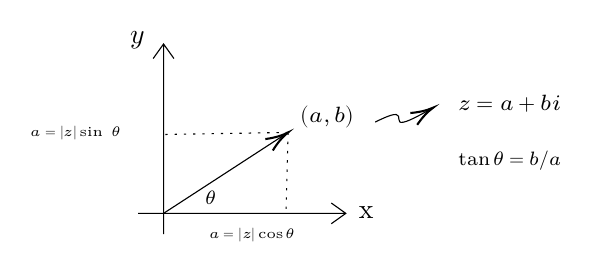
\begin{tikzpicture}[x=0.75pt,y=0.75pt,yscale=-1,xscale=1]
%uncomment if require: \path (0,385); %set diagram left start at 0, and has height of 385

%Shape: Axis 2D [id:dp019899055915183705] 
\draw  (186,175.6) -- (286,175.6)(198.2,94) -- (198.2,185.6) (279,170.6) -- (286,175.6) -- (279,180.6) (193.2,101) -- (198.2,94) -- (203.2,101)  ;
%Straight Lines [id:da24458232880287722] 
\draw    (198.2,175.6) -- (256.52,137.69) ;
\draw [shift={(258.2,136.6)}, rotate = 146.98] [color={rgb, 255:red, 0; green, 0; blue, 0 }  ][line width=0.75]    (10.93,-3.29) .. controls (6.95,-1.4) and (3.31,-0.3) .. (0,0) .. controls (3.31,0.3) and (6.95,1.4) .. (10.93,3.29)   ;
%Straight Lines [id:da3272591109121279] 
\draw  [dash pattern={on 0.84pt off 2.51pt}]  (258.2,136.6) -- (257.2,174.6) ;
%Straight Lines [id:da896305170387582] 
\draw  [dash pattern={on 0.84pt off 2.51pt}]  (258.2,136.6) -- (198.2,137.6) ;
%Shape: Boxed Bezier Curve [id:dp47020263210839053] 
\draw    (300.2,131.6) .. controls (323.84,119.78) and (298,141.92) .. (326.84,125.38) ;
\draw [shift={(328.2,124.6)}, rotate = 149.86] [color={rgb, 255:red, 0; green, 0; blue, 0 }  ][line width=0.75]    (10.93,-3.29) .. controls (6.95,-1.4) and (3.31,-0.3) .. (0,0) .. controls (3.31,0.3) and (6.95,1.4) .. (10.93,3.29)   ;

% Text Node
\draw (291,171) node [anchor=north west][inner sep=0.75pt]   [align=left] {x};
% Text Node
\draw (181,86.4) node [anchor=north west][inner sep=0.75pt]    {$y$};
% Text Node
\draw (339,117.4) node [anchor=north west][inner sep=0.75pt]  [font=\footnotesize]  {$z=a+bi$};
% Text Node
\draw (263,122.4) node [anchor=north west][inner sep=0.75pt]  [font=\footnotesize]  {$( a,b)$};
% Text Node
\draw (217,163.4) node [anchor=north west][inner sep=0.75pt]  [font=\scriptsize]  {$\theta $};
% Text Node
\draw (219,181.4) node [anchor=north west][inner sep=0.75pt]  [font=\tiny]  {$a=|z|\cos \theta $};
% Text Node
\draw (133,132.4) node [anchor=north west][inner sep=0.75pt]  [font=\tiny]  {$a=|z|\sin \ \theta $};
% Text Node
\draw (339,144.4) node [anchor=north west][inner sep=0.75pt]  [font=\scriptsize]  {$\tan \theta =b/a$};


\end{tikzpicture}
    \end{center}
\end{itemize}

则由三角函数的定义知:$z$的\textit{实部(real part)}$Re(z)$和\textit{虚部(imaginary part)}$Im(z)$ 可通过其模长$|z|$和其\textit{幅角(argument)} $\theta=arg\,z$ 表示如下\[\left\{\begin{array}{c}
       Re(z)=a=|z|\cos{\theta}\\
      Im(z)=b=|z|\sin{\theta}
\end{array}\right.\]

其中幅角$\theta=arg\,z$由$\tan\theta=\frac{b}{a}$给出. 即有$z=|z|(\cos{\theta}+i\sin{\theta})$. 反之,给出一表达$\rho(\cos{\theta}+i\sin{\theta})$,则它代表一复数,其模长为$\rho$,其实部和虚部分别由$\rho\cos{\theta}$和$\rho\sin{\theta}$给出. 在极表示下,复数乘(除)法的几何意义较易直观而得. 

\begin{itemize}
    \item \textit{复数乘法的几何意义:} 给定两非零复数$z=\rho(\cos{\alpha}+i\sin{\alpha})$ 和$w=r(\cos{\beta}+i\sin{\beta})$. 按复数的乘法运算规则,再结合三角函数的\textit{加法定理},得
    \[zw=\rho r(\cos{(\alpha+\beta})+i\sin{(\alpha+\beta)}\]
    同理,若$w\neq 0$,则$z/w=\frac{\rho}{r}(\cos{(\alpha-\beta})+i\sin{(\alpha-\beta)}$. 由此即明复数乘(除)法的几何意义. 
    \begin{center}
        

\tikzset{every picture/.style={line width=0.75pt}} %set default line width to 0.75pt        

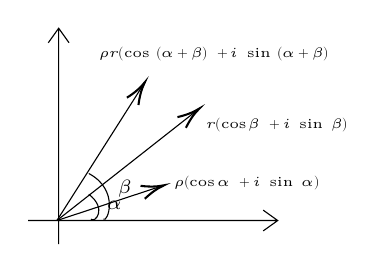
\begin{tikzpicture}[x=0.75pt,y=0.75pt,yscale=-1,xscale=1]
%uncomment if require: \path (0,385); %set diagram left start at 0, and has height of 385

%Shape: Axis 2D [id:dp019899055915183705] 
\draw  (258,195.25) -- (378.2,195.25)(272.66,102.6) -- (272.66,206.6) (371.2,190.25) -- (378.2,195.25) -- (371.2,200.25) (267.66,109.6) -- (272.66,102.6) -- (277.66,109.6)  ;
%Straight Lines [id:da24458232880287722] 
\draw    (271.81,195.25) -- (321.62,178.86) ;
\draw [shift={(323.52,178.24)}, rotate = 161.79] [color={rgb, 255:red, 0; green, 0; blue, 0 }  ][line width=0.75]    (10.93,-3.29) .. controls (6.95,-1.4) and (3.31,-0.3) .. (0,0) .. controls (3.31,0.3) and (6.95,1.4) .. (10.93,3.29)   ;
%Straight Lines [id:da16632308178635347] 
\draw    (271.81,195.25) -- (338.94,142.47) ;
\draw [shift={(340.52,141.24)}, rotate = 141.83] [color={rgb, 255:red, 0; green, 0; blue, 0 }  ][line width=0.75]    (10.93,-3.29) .. controls (6.95,-1.4) and (3.31,-0.3) .. (0,0) .. controls (3.31,0.3) and (6.95,1.4) .. (10.93,3.29)   ;
%Curve Lines [id:da7195309903411762] 
\draw    (287.2,182.6) .. controls (296.2,189.6) and (290.2,196.6) .. (288.2,194.6) ;
%Straight Lines [id:da4068358889414354] 
\draw    (271.81,195.25) -- (313.13,130.29) ;
\draw [shift={(314.2,128.6)}, rotate = 122.46] [color={rgb, 255:red, 0; green, 0; blue, 0 }  ][line width=0.75]    (10.93,-3.29) .. controls (6.95,-1.4) and (3.31,-0.3) .. (0,0) .. controls (3.31,0.3) and (6.95,1.4) .. (10.93,3.29)   ;
%Curve Lines [id:da27962537380618535] 
\draw    (287.2,172.6) .. controls (302.2,180.6) and (296.2,196.6) .. (294.2,194.6) ;

% Text Node
\draw (295,184.4) node [anchor=north west][inner sep=0.75pt]  [font=\scriptsize]  {$\alpha $};
% Text Node
\draw (300,174.4) node [anchor=north west][inner sep=0.75pt]  [font=\scriptsize]  {$\beta $};
% Text Node
\draw (327,172.4) node [anchor=north west][inner sep=0.75pt]  [font=\tiny]  {$\rho (\cos \alpha \ +i\ \sin \ \alpha )$};
% Text Node
\draw (342.52,144.64) node [anchor=north west][inner sep=0.75pt]  [font=\tiny]  {$r(\cos \beta \ +i\ \sin \ \beta )$};
% Text Node
\draw (291,110.4) node [anchor=north west][inner sep=0.75pt]  [font=\tiny]  {$\rho r(\cos \ ( \alpha +\beta ) \ +i\ \sin \ ( \alpha +\beta )$};


\end{tikzpicture}
    \end{center}
\end{itemize}

\begin{itemize}
    \item \textit{复数的复指数(complex exponential)表示:} 由著名的\textit{欧拉公式(Euler formula)}:$e^{i\theta}=\cos\theta+i\sin\theta$,可将复数的极表示转化为下面的复指数表示\[z=\rho(\cos\theta+i\sin\theta)=\rho e^{i\theta}\qquad \textit{其中}\,\,\rho=|z|;\,\,\theta=arg\,z\]
\end{itemize}

(复)指数函数最重要的性质是,\textit{它将加法转变为乘法}(其逆对数函数则将乘法转变为加法),即有$e^{i(\alpha+\beta)}=e^{i\alpha}e^{i\beta}$. 则不难看出,该运算性质恰好对应于复数乘法对应的旋转意义:$zw=\rho e^{i\alpha}\,re^{i\beta}=\rho r e^{i(\alpha+\beta)}$

\vspace{4pt}

\textbf{注记 1.2} \textit{对任意$\theta\in \mathbb{R}$,$|e^{i\theta}|=1$,故平面单位圆(unit circle)可用复数表示如下}\[S^{1}:=\{(x,y)\in \mathbb{R}^{2}\mid x^{2}+y^{2}=1\}=\{z\in \mathbb{C}\mid z\Bar{z}=1\}=\{e^{i\theta}\mid \theta\in [0,\,2\pi)\}\]


\section{逻辑符号与命题逻辑}

命题可通过逻辑符号合成或转变为其它命题,或者说,命题是通过逻辑符号进行“运算”的. 常用的逻辑符号有
\begin{enumerate}
    \item \textit{或(or)} $\lor$
    \item \textit{且(and)} $\land$
    \item \textit{否(there is no)} $\neg$
    \item \textit{至少存在(there exists at least one)} $\exists$
    \item \textit{存在唯一(there exists one and only one)} $\exists!$
    \item \textit{对所有的(for all)} $\forall$
     \item \textit{蕴含、推出 (implies)} $\Rightarrow$ 
\end{enumerate}

\textbf{定义 2.1} 如果对两命题$p,q$,有$p\Rightarrow q$ 且 $q\Rightarrow p$,则称$p$和$q$\textit{等价(equivalent)},或$p$\textit{当且仅当(if and only if,\,iff)},记为$p\Longleftrightarrow q$. 

\vspace{3pt}

我们用$“1”$表示命题为真,用$“0”$表示命题为假. 复合命题的真假可用\textit{真值表(truth value table)} 来判定,其基本类型给出如下:
\begin{center}
    
    \begin{tabular}{c|c|c|c|c|c|c}
       $p$ & $q$ & $\neg p$ & $p\land q$ & $p\lor q$ & $p\Rightarrow q$ & $\neg p\lor q$\\
       \hline
       $0$ & $0$ & $1$ & $0$ & $0$ & $1$ & $1$ \\
       \hline
       $1$ & $0$ & $0$ & $0$ & $1$ & $0$ & $0$ \\
       \hline 
       $0$ & $1$ & $1$ & $0$ & $1$ & $1$ & $1$ \\
       \hline
       $1$ & $1$ & $0$ & $1$ & $1$ & $1$ & $1$ \\

    \end{tabular}

\end{center}

上表说明:
\begin{enumerate}
    \item $p$为真(假)当且仅当$\neg p$为假(真).
    \item $p\land q$ 为真当且仅当$p$和$q$同时为真. 
    \item $p\lor q$为假当且仅当$p$和$q$同时为假.
    \item $p\Rightarrow q$ 为假当且仅当$p$真$q$假.(\textit{即假命题可推出或真或假的命题,单真命题只能推出真命题})
    \item 注意到$p\Rightarrow q$ 和$\neg p\lor q$的真值属性相同,这说明两者是等价的. 即:若$p$为真,则“$p$推出$q$” 等价于 “如$p$非假则必有$q$”. 
    \end{enumerate}

\textbf{练习 2.1} 写出$p\Longleftrightarrow 
 q$的真值表. 

\vspace{3pt}

\textbf{命题 2.1} 命题$p\Rightarrow q$ 与其\textit{逆否命题(contrapositive)} $\neg q\Rightarrow \neg p$等价. 

\vspace{3pt}

\textbf{证明:} 由下真值表可知命题成立:

\begin{center}
    \begin{tabular}{c|c|c|c}
        $p$ & $q$ & $p\Rightarrow q$ & $\neg q\Rightarrow \neg p$\\
\hline
       $0$ & $0$ & $1$ & $1$\\
       \hline
       $1$ & $0$  & $0$ & $0$\\
        \hline
       $0$ & $1$  & $1$ & $1$\\
        \hline
       $1$ & $1$ & $1$ & $1$\\
    \end{tabular}
\end{center}

类似地,利用真值表,可证以下命题成立.

\vspace{3pt}

\textbf{命题 2.2} 关于命题的否定形式,我们有以下结论
\begin{enumerate}
    \item $\neg(\neg p)\Longleftrightarrow p$. \textit{(双重否定)}
    \item $\left\{\begin{array}{c}
          \neg (p\lor q)\quad \Longleftrightarrow \quad \neg p\land \neg q \\
          \neg(p\land q)\quad \Longleftrightarrow \quad \neg p\lor \neg q
    \end{array}\right.$ \textit{(对偶律,或德摩根律)}   
\end{enumerate}

\textbf{命题 2.3} 对涉及\textit{全称量词}$\forall$和\textit{存在量词} $\exists$ 的命题,其否定形式为 (更一般的\textit{对偶律})\[\left\{\begin{array}{c}
        \neg(\forall x,\,\textit{使得}\,p(x))\quad \Longleftrightarrow\quad 
    \exists\,x,\,\textit{使得}\,\neg\,p(x)  \\
     \neg(\exists x,\,\textit{使得}\,p(x))\quad \Longleftrightarrow\quad 
    \forall\,x,\,\textit{使得}\,\neg\,p(x)
    \end{array}\right.\]

其中$p(x)$是涉及$x$的命题.

\vspace{3pt}

\textbf{证明:} $\forall x,\,\textit{使得}\,p(x)$ 相当于$\land_{x}\,p(x)$. 由上命题中的$2$知,其否定为$\lor_{x}\,\neg p(x)$,它为真当且仅当存在$\neg p(x)$为真;同理,$\exists x,\,\textit{使得}\,p(x)$ 相当于$\lor_{x}\,p(x)$. 由上命题中的$2$知,其否定为$\land_{x}\,\neg p(x)$,它为真当且仅当所有$\neg p(x)$为真. \qquad$\square$

\vspace{4pt}

\textbf{例 2.1} 用逻辑符号及其规则,可将\textit{命题 1.1} 重新表述为:“$\forall\delta>0$,长度为$
\delta$的区间$I\subseteq \mathbb{R}$内有无穷多个有理数.” 根据上述命题,其否定形式为:$\exists\delta>0$,使得长度为$\delta$的区间$I\subseteq \mathbb{R}$中只有有限个有理数.

\vspace{3pt}

\textbf{例 2.2} 对$\sqrt{2}$是无理数的经典证明中,我们用到命题:“如$p^{2}$是偶数,则$p$本身是偶数.” 它等价于其逆否命题:“如$p$是奇数,则$p^{2}$是奇数. ” 用反证法证明命题,则相当于证明了其逆否命题,从而得到一个矛盾(不可能命题).

\vspace{3pt}

\textbf{例 2.3} 一个函数$f(x)$ 称为是\textit{周期函数(periodic function)} 如下命题成立

\vspace{3pt}

\qquad $\exists\, T>0$,$\forall\,x\in D(f)$,成立$f(x+T)=f(x)$

\vspace{3pt}

满足上命题的最小$T$,称为$f$的\textit{最小正周期}. 则$f$是非周期函数应描述如下

\vspace{3pt}

\qquad $\forall\,T>0,\,\exists\,x\in D(f)$,
使得$f(x+T)\neq f(x)$

\vspace{3pt}

\textbf{例 2.4} 对集合$X,Y$,包含关系$X\subseteq Y$可描述为:“$\forall\,x\in X$,\,皆有\,$x\in Y$.” 则其否命题:“$\exists\,x\in X$,\,使得\,$x\notin Y$” 便是关系$X\nsubseteq Y$的命题描述.

\vspace{3pt}

\textbf{例 2.5} 给出一数列$\{a_{n}\}$,它是\textit{有界(bounded)}的当且仅当:$\exists\,M>0,\,\forall\,n$,使得$|a_{n}|\leq M$. 则根据\textit{对偶原则},数列$\{a_{n}\}$\textit{无界(unbounded)}的描述命题是:$\forall\,M>0,\,\exists\,n$,使得$|a_{n}|>M$.

\vspace{4pt}

更一般地,对命题:$Q_{1}p_{1}Q_{2}p_{2}\cdots Q_{n}p_{n},\,\textit{使得}\,p_{n+1}$ (其中$Q_{i}$为$\forall$或$\exists$,\,$p_{i}$\,为命题),其否定命题由\textit{对偶原则(duality principle)} 给出:

\vspace{3pt}

\qquad \uwave{将诸$Q_{i}$中的$\forall (\exists)$改成$\exists (\forall)$,并将最后的$p_{n+1}$改成其否定形式}.



\newpage

\section{映射与函数}

高中时,我们将一函数记做$y=f(x)$,其中$x\in D$称为自变量,其取值范围$D\subseteq\mathbb{R}$称为函数的\textit{定义域(domain)},而$y$称为变量,其取值范围$y\in R\subseteq \mathbb{R}$称为函数的\textit{值域(range)}. $f$ 指的是函数(function)的作用规则,即对任意$x\in D$,存在唯一$y\in R$,通过$f$的指认,与$x$相对应. 

\vspace{4pt}

\textbf{注记 3.1} \textit{从动态视角来看,$x$的变化引起了$y$的变化,即“函数是变化着的数”. 若$x$的变化未引起$y$取值的变化,则函数是常数值函数. 将$x$ 看成是“时间”变量,则$(x,y)$的取值描绘出平面上的一条轨迹,称为函数$f$的图形(graph),记为$G(f)$,即有}\[G(f):=\{(x,y)\mid x\in D,\,y=f(x)\}\subseteq \mathbb{R}^{2}\]

上面函数的概念其实是更广泛的映射概念的特例.

\vspace{4pt}

\textbf{定义 3.1} 设$X, Y$ 为两非空集合,若$T$是一个从$X$的元素到$Y$的元素的一个对应法则,它满足:对任意$x\in X$,存在唯一的$y\in Y$与之对应,则称$T$ 是从$X$到$Y$的\textit{映射(mapping)},记为$T: X\longrightarrow Y\quad x\longmapsto y=T(x)$. 另称$y=T(x)$是$x$在$T$作用下的\textit{象(image)},$x$是$y$在$T$下的\textbf{一个}\textit{原象(preimage)}. 此时,$X$称为$T$的定义域,且$T$的象(或值域)$R(T)$定义为 $R(T):=\{y\in Y\mid y=T(x), \,x\in X\}$.

\vspace{4pt}

\textbf{定义 3.2} 若$f$是从$D\subseteq \mathbb{R}$到$\mathbb{R}$的一个映射,则称$f$ \textit{是一元实函数(在本课程中,简称为函数).} 

\vspace{3pt}

\textbf{注记 3.2}\textit{以后会考虑从平面$\mathbb{R}^{2}:=\{(x,y)\mid x,y\in\mathbb{R}\}$ 或空间$\mathbb{R}^{3}:=\{(x,y,z)\mid x,y,z\in\mathbb{R}\}$的子集到$\mathbb{R}$的映射,称为是二元实函数或三元实函数;也会考虑到从复数域$\mathbb{C}$的子集到$\mathbb{C}$映射,称为是一元复变函数. 类似地,可考虑多元复变函数等. }

\vspace{4pt}

\textbf{定义 3.3} 一映射$T:\,X\longrightarrow Y$ 称为是\textit{单射(injection)} 如它满足性质:

\vspace{3pt}

\qquad $\forall\,x,y\in X$,如$T(x)=T(y)$,则必有$x=y$.

\vspace{3pt}

即不存在两不同的元素被映为同一元素. 单射也被称作是\textit{“一一映射”(one-to-one mapping)}. 

\vspace{3pt}

\textbf{定义 3.4} 一映射$T:\,X\longrightarrow Y$ 称为是\textit{满射(surjection)} 如它满足性质:

\vspace{3pt}

\qquad $\forall\,y\in Y$,\,$\exists\,x\in 
 X$,使得$y=T(x)$. 

 \vspace{3pt}

 即$Y$中的任意元素都是$T$的象. 满射也被称作是\textit{映上的(onto)}.

\vspace{3pt}

\textbf{定义 3.5} $T:\,X\longrightarrow Y$ 称为是\textit{双射(bijection)} 如它既是单射又是满射. 我们也常说一个双射$T:X\longrightarrow Y$建立了集合$X$和集合$Y$之间的一个\textit{一一对应(one-to-one correspondence)}.

\vspace{3pt}


\textbf{例 3.1} $f: \mathbb{R}\longrightarrow \mathbb{R}\quad x\longmapsto x^{2}$ 是映射,其值域是$\mathbb{R}_{\geq 0}:=\{y\in \mathbb{R}\mid y\geq 0\}$. 它不是从$\mathbb{R}$到$\mathbb{R}$的满射,但是从$\mathbb{R}$到$\mathbb{R}_{\geq 0}$的满射,因为每个非负实数都可开平方根. 它也不是单射,因为$-1$和$1$都是$1$的原象. 

\vspace{4pt}

\textbf{例 3.2} 复指数函数$e^{i\theta}$ 是从$\mathbb{R}$到复平面$\mathbb{C}$的一个映射. $T:\,\mathbb{R}\longrightarrow\mathbb{R}$,它满足\[T(x+y)=T(x)\,T(y)\]

显然$T$ 不是满射,其值域是复平面中的单位圆$S^{1}$. 故$T$是从$\mathbb{R}$到$S^{1}$的满射. 它也不是单射,由三角函数的周期性可知$T(x+2k\pi)=e^{i(x+2k\pi)}=$\[=\cos{(x+2k\pi)}+i\sin{(x+2k\pi)}=e^{ix}=T(x)\quad \forall\,k\in\mathbb{Z}\]

但若将定义域取为$D:=[0,2\pi)$ 则$T$是从$D$到$S^{1}$的单射,此时$T$也是满射,故$T$建立了$D$中元素同$S^{1}$中元素之间的一个一一对应. 

\vspace{4pt}

\textbf{例 3.3} 一个映射$T:\,\mathbb{R}\longrightarrow \mathbb{R}$称为是\textit{线性的(linear)} 如果\begin{enumerate}
    \item $T(x+y)=T(x)+T(y),\,\,\forall x,y\in\mathbb{R}$;
    \item $T(kx)=kT(x),\,\,\forall k\in \mathbb{R}$
\end{enumerate}

显然,我们熟知的一次函数$y=f(x)=ax\,\,(a\in\mathbb{R})$ 是线性的,故它也被称为是线性函数. 反之,若$T$是从$\mathbb{R}$到$\mathbb{R}$的线性映射,则对任意非零实数$x$,由性质$2$知$T(x)=T(x\cdot 1)=xT(1)$,设$T(1)=a$,则$T
(x)=ax$.

\vspace{3pt}

\textbf{练习 3.1} 若$T:\mathbb{R}\to\mathbb{R}$是线性的,证明$T$是单射当且仅当:若$T(x)=0$,则$x=0$. 

\vspace{3pt}

\textbf{练习 3.2} 若$T:\mathbb{R}\to\mathbb{R}$是线性的,证明$T$是单射当且仅当$T$是满射的. 

\vspace{3pt}

\textbf{例 3.4} 对集合$X,Y$,考虑其乘积$X\times Y$,我们有从$X\times Y$到$X$和$Y$的\textit{投影映射(projection)}\[pr_{X}:\,X\times Y\longrightarrow X\quad (x,y)\longmapsto x\]\[pr_{Y}:\,X\times Y\longrightarrow Y\quad (x,y)\longmapsto y\]

投影映射是满射,但一般不是单射. 

\vspace{3pt}

\textbf{思考 3.1} 当$X=Y=\mathbb{R}$,如何使$pr_{X}$或$pr_{Y}$成为线性的?

\vspace{3pt}

\textbf{练习 3.3} 对一函数$f:\mathbb{R}\longrightarrow \mathbb{R}$,记其图像为$G(f):=\{(x,y)\mid y=f(x),\,x\in D\}$. 则可将投影$pr:\,\mathbb{R}\times \mathbb{R}\longmapsto\mathbb{R}\quad (x,y)\longmapsto y$ 限制到图像$G(f)$上,得到如下映射\[pr|_{G(f)}:\,G(f)\longrightarrow \mathbb{R}\qquad (x,y)\longmapsto y\]

证明:$f$ 是满的当且仅当$pr|_{G(f)}$也是满的.

\vspace{4pt}

\textbf{定义 3.6} 设$T:\,X\longrightarrow Y$ 是映射,则对其象$R(T)$中的任意元素$y$,如果其原象$x\in X$(即满足$T(x)=y$的$x$)是\textbf{唯一}确定的,则由映射的定义知下面对应规则定义了一映射\[S: R(T)\longrightarrow X\qquad y\longmapsto x\,\,(T(x)=y)\]

映射$S$称为$T$的\textit{逆映射(inverse mapping)},常记作$T^{-1}$. $T^{-1}$的定义(值)域是$T$的值(定义)域. 

\vspace{3pt}

若将$T$特殊化为一元实函数,则其逆便是我们熟知的反函数的概念. 一函数和它的反函数的图像关于直线$y=x$对称. 

\vspace{3pt}

\textbf{例 3.5} 函数$y=\sin{x}$是$\mathbb{R}$上的周期函数,其最小正周期是$2\pi$. 将其自然定义域$\mathbb{R}$缩小为$\left[-\frac{\pi}{2},\,\frac{\pi}{2}\right]$,则得到从$\left[-\frac{\pi}{2},\,\frac{\pi}{2}\right]$到$[-1,1]$的双射,则将其逆定义为\textit{反正弦函数}\[y=\arcsin{x}\quad [-1,1]\longrightarrow \left[-\frac{\pi}{2},\,\frac{\pi}{2}\right]\]

则有恒等式$\sin{(\arcsin{y})}=y,\,\,y\in[-1,1]$;\,\,\,$\arcsin{(\sin{x})}=x,\,\,x\in\left[-\frac{\pi}{2},\,\frac{\pi}{2}\right]$.

\vspace{3pt}

同理,可定义\textit{反余弦函数}$y=\arccos{x}:\quad [-1,1]\longrightarrow[0,\pi]$,以及\textit{反正切函数} $y=\arctan\,x:\quad (-\infty,\,\infty)\longrightarrow \left(-\frac{\pi}{2},\,\frac{\pi}{2}\right)$ 等等.

\vspace{4pt}


\textbf{定义 3.7} 设$f: U\longrightarrow Y$和$g: X\longrightarrow V$是两映射,如果$R(g)\cap D(f)\neq \emptyset$,则可定义$f$与$g$的\textit{复合映射(composite map)}如下\[f\circ g:\,X^{*}\longrightarrow Y\qquad (f\circ g)(x):=f[g(x)],\,x\in X^{*}\]

其中$X^{*}=D(f\circ g):=\{x\in X\mid g(x)\in D(f)\}\subseteq X$. 

\vspace{3pt}


\textbf{练习 3.4} 对映射$T$及其逆映射$T^{-1}$,证明有$T\circ T^{-1}=I|_{R(T)};\,\, T^{-1}\circ T=I|_{D(T)}$,其中$I$代表恒等映射,即满足$I(x)=x$的映射. 

\vspace{3pt}

\textbf{例 3.6} 若$f$和$g$是函数,则其复合$y=f[g(x)]$ 是通过\textit{中间变量} $u=g(x)$ 将$y=f(u)$和$u=g(x)$复合而成的.

\vspace{3pt}

\textbf{例 3.7} 一般的一次函数$y=ax+b$可看成是由$y=x+b$ (平移) 和$u=ax$(伸缩)复合而成. 

\vspace{3pt}

\textbf{练习 3.5} 一次函数之间的复合所得的任然是一次函数. 

\vspace{3pt}

\textbf{例 3.8} 有时也考虑函数与其自身的连续复合,比如$f^{2}(x)=f(f(x))$,\,$f^{3}(x)=f(f(f(x))),\cdots$,$f^{n}(x)=\underbrace{f(f(f\cdots f(x))}_{n}$


\section{初等函数,函数的趣例}

下面五类函数称为\textit{基本初等函数(basic elementary functions)}
\begin{enumerate}
    \item \textit{幂函数}:$y=x^{a}\,(a\in \mathbb{R})$. 常数函数$y=c$看成是其特例. 
    \item \textit{指数函数}:$y=a^{x}\,(a>0,\,a\neq 1)$.
    \item \textit{对数函数}:$y=\log_{a}\,x\,(a>0,\,a\neq 1)$. 当$a=e=2.71828\cdots$时,记为$y=\ln{x}$.
    \item \textit{三角函数}:$y=\sin{x}$,\,$y=\cos{x}$,\,$y=\tan\,x$ 等.
    \item \textit{反三角函数}:$y=\arcsin{x}$,\,$y=\arccos{x}$,\,$y=\arctan\,x$ 等.
\end{enumerate}

\textbf{定义 4.1} 由基本初等函数经过有限次四则运算与复合运算所产生的函数称为\textit{初等函数}. 

\vspace{4pt}

\textbf{例 4.1} $\displaystyle y=e^{-x^{2}}+\arctan\frac{1}{x}$;$\displaystyle y=\frac{\ln{(x+\sqrt{1+x^{2}})}-3e^{-x^{2}}}{\arctan\,(1+\cos^{2}x)}$ 都是初等函数.

\vspace{4pt}

\textbf{例 4.2} 由基本幂函数$\{1,x,x^{2},\cdots,x^{n}\}$ 和常数函数通过$“+”$ 和 $“\times”$ 可生成\textit{多项式函数(polynomial function)}\[y=a_{0}+a_{1}x+a_{2}x^{2}+\cdots+a_{n}x^{n}\quad a_{i}\in \mathbb{R}\]

若$a_{n}\neq 0$,则称其为(中心为$0$的)$n$次(一元)多项式. 有时将多项式写称下面的形式,称其是中心为$a$的多项式\[y=a_{0}+a_{1}(x-a)+a_{2}(x-a)^{2}+\cdots+a_{n}(x-a)^{n}\]

当然,非零中心的多项式总可以写成以零为中心的形式.

\vspace{3pt}

\textbf{例 4.3} \textit{有理函数(rational function)}定义为两多项式函数之商,即具有如下形式的函数\[y=\frac{a_{0}+a_{1}x+a_{2}x^{2}+\cdots+a_{n}x^{n}}{b_{0}+b_{1}x+b_{2}x^{2}+\cdots+b_{m}x^{m}}\]

其自然定义域是所有使得分母不为零的实数. 

\vspace{3pt}

一般而言,分段函数不是初等函数,因为不同区间上定义的函数无法用法统一地用解析式来表达. 但对有些函数,比如下例中的函数,分段只是为了表述方便,但事实上可用一个解析式来表达,故它是初等函数.


\vspace{3pt}

\textbf{例 4.4} $y=|x|=\left\{\begin{array}{c}
     x\qquad x\geq 0  \\
     -x\qquad x<0
\end{array}\right.$  它可表达为$y=|x|=\sqrt{x^{2}}$

\vspace{3pt}

下面是非初等的分段函数的重要例子.

\vspace{3pt}

\textbf{例 4.5} \textit{符号函数(sign function)}:$sgn\,x:=\left\{\begin{array}{c}
     1 \qquad x>0 \\
     0\qquad x=0\\
     -1\qquad x<0
\end{array}\right.$ 其图像给出如下
\begin{center}
    

\tikzset{every picture/.style={line width=0.75pt}} %set default line width to 0.75pt        

\begin{tikzpicture}[x=0.75pt,y=0.75pt,yscale=-1,xscale=1]
%uncomment if require: \path (0,385); %set diagram left start at 0, and has height of 385

%Shape: Axis 2D [id:dp29138516508888435] 
\draw  (200,208.6) -- (372.2,208.6)(286.2,132.6) -- (286.2,270) (365.2,203.6) -- (372.2,208.6) -- (365.2,213.6) (281.2,139.6) -- (286.2,132.6) -- (291.2,139.6)  ;
%Straight Lines [id:da9137768256652159] 
\draw    (286,182) -- (361.2,181.6) ;
%Straight Lines [id:da9195039155431399] 
\draw    (209.2,235.6) -- (287.2,235.6) ;

% Text Node
\draw (373,210.4) node [anchor=north west][inner sep=0.75pt]    {$x$};
% Text Node
\draw (267,126.4) node [anchor=north west][inner sep=0.75pt]    {$y$};
% Text Node
\draw (288.2,212) node [anchor=north west][inner sep=0.75pt]  [font=\footnotesize]  {$0$};
% Text Node
\draw (282,178.4) node [anchor=north west][inner sep=0.75pt]    {$\circ $};
% Text Node
\draw (282,231.4) node [anchor=north west][inner sep=0.75pt]    {$\circ $};
% Text Node
\draw (281,198.4) node [anchor=north west][inner sep=0.75pt]  [font=\Large]  {$\centerdot $};


\end{tikzpicture}
\end{center}

\textbf{例 4.6} \textit{$\delta$ 函数,或脉冲函数}:$\delta\,(x)=\left\{\begin{array}{c}
     \infty\quad x=0  \\
     0\quad x\neq 0
\end{array}\right.$ (另外,它的图像与$x$轴所围“面积”为1). 它是一个奇怪的函数,但却无比常见. 对其严格处理须用到数学中的\textit{“广义函数”,或“分布”(distribution)理论}. 形式上,$\delta\,(x)$可看成是$sign\,x$的导函数.

\vspace{3pt}

\textbf{例 4.7} \textit{取整函数}:$y=[x]=n,\,n\leq x<n+1,\,n\in\mathbb{Z}$. 即$[x]$是不超过$x$的最大整数. 其图像给出如下
\begin{center}
    

\tikzset{every picture/.style={line width=0.75pt}} %set default line width to 0.75pt        

\begin{tikzpicture}[x=0.75pt,y=0.75pt,yscale=-1,xscale=1]
%uncomment if require: \path (0,385); %set diagram left start at 0, and has height of 385

%Shape: Axis 2D [id:dp9850704200198039] 
\draw  (146,177.7) -- (473.2,177.7)(310.25,52.6) -- (310.25,286) (466.2,172.7) -- (473.2,177.7) -- (466.2,182.7) (305.25,59.6) -- (310.25,52.6) -- (315.25,59.6) (350.25,172.7) -- (350.25,182.7)(390.25,172.7) -- (390.25,182.7)(430.25,172.7) -- (430.25,182.7)(270.25,172.7) -- (270.25,182.7)(230.25,172.7) -- (230.25,182.7)(190.25,172.7) -- (190.25,182.7)(305.25,137.7) -- (315.25,137.7)(305.25,97.7) -- (315.25,97.7)(305.25,217.7) -- (315.25,217.7)(305.25,257.7) -- (315.25,257.7) ;
\draw   (357.25,189.7) node[anchor=east, scale=0.75]{1} (397.25,189.7) node[anchor=east, scale=0.75]{2} (437.25,189.7) node[anchor=east, scale=0.75]{3} (277.25,189.7) node[anchor=east, scale=0.75]{-1} (237.25,189.7) node[anchor=east, scale=0.75]{-2} (197.25,189.7) node[anchor=east, scale=0.75]{-3} (307.25,137.7) node[anchor=east, scale=0.75]{1} (307.25,97.7) node[anchor=east, scale=0.75]{2} (307.25,217.7) node[anchor=east, scale=0.75]{-1} (307.25,257.7) node[anchor=east, scale=0.75]{-2} ;
%Straight Lines [id:da49885838538616345] 
\draw [line width=3]    (310.25,177.7) -- (348.2,177.6) ;
%Shape: Circle [id:dp5655926580591619] 
\draw   (348.2,177.6) .. controls (348.19,175.93) and (349.53,174.6) .. (351.19,174.62) .. controls (352.86,174.64) and (354.22,176) .. (354.23,177.67) .. controls (354.24,179.33) and (352.9,180.67) .. (351.24,180.65) .. controls (349.57,180.63) and (348.21,179.27) .. (348.2,177.6) -- cycle ;
%Straight Lines [id:da5764484765904125] 
\draw [line width=3]    (347.79,138.66) -- (385.74,138.56) ;
%Shape: Circle [id:dp6513046619180758] 
\draw   (385.74,138.56) .. controls (385.72,136.65) and (387.26,135.12) .. (389.17,135.14) .. controls (391.09,135.16) and (392.65,136.73) .. (392.66,138.64) .. controls (392.68,140.55) and (391.14,142.08) .. (389.23,142.06) .. controls (387.31,142.04) and (385.75,140.47) .. (385.74,138.56) -- cycle ;
%Straight Lines [id:da8180732391061305] 
\draw [line width=3]    (390.25,99.7) -- (428.2,99.6) ;
%Shape: Circle [id:dp14318816157729297] 
\draw   (428.2,99.14) .. controls (428.18,97.48) and (429.52,96.15) .. (431.17,96.17) .. controls (432.83,96.19) and (434.18,97.55) .. (434.2,99.2) .. controls (434.21,100.86) and (432.88,102.19) .. (431.22,102.17) .. controls (429.56,102.15) and (428.21,100.8) .. (428.2,99.14) -- cycle ;
%Straight Lines [id:da5571134410678611] 
\draw [line width=3]    (269.25,217.7) -- (307.2,217.6) ;
%Straight Lines [id:da07314261124982013] 
\draw [line width=3]    (231.25,259.7) -- (269.2,259.6) ;
%Shape: Circle [id:dp5189118937347017] 
\draw   (405.74,158.56) .. controls (405.72,156.65) and (407.26,155.12) .. (409.17,155.14) .. controls (411.09,155.16) and (412.65,156.73) .. (412.66,158.64) .. controls (412.68,160.55) and (411.14,162.08) .. (409.23,162.06) .. controls (407.31,162.04) and (405.75,160.47) .. (405.74,158.56) -- cycle ;
%Shape: Circle [id:dp6185614660830356] 
\draw   (307.2,217.6) .. controls (307.19,215.69) and (308.72,214.15) .. (310.64,214.18) .. controls (312.55,214.2) and (314.11,215.76) .. (314.13,217.68) .. controls (314.14,219.59) and (312.6,221.12) .. (310.69,221.1) .. controls (308.78,221.08) and (307.21,219.51) .. (307.2,217.6) -- cycle ;
%Shape: Circle [id:dp10742290895436923] 
\draw   (269.2,259.6) .. controls (269.19,257.69) and (270.72,256.15) .. (272.64,256.18) .. controls (274.55,256.2) and (276.11,257.76) .. (276.13,259.68) .. controls (276.14,261.59) and (274.6,263.12) .. (272.69,263.1) .. controls (270.78,263.08) and (269.21,261.51) .. (269.2,259.6) -- cycle ;

% Text Node
\draw (312.25,181.1) node [anchor=north west][inner sep=0.75pt]  [font=\footnotesize]  {$0$};


\end{tikzpicture}
\end{center}

\textbf{例 4.7$^{\prime}$} \textit{非负小数部分函数}:$y=(x)=x-[x]$.

\vspace{3pt}

\textbf{例 4.8} \textit{迪利克雷(Dirichlet)函数}: $D(x):=\left\{\begin{array}{c}
     1\qquad x\in \mathbb{Q}  \\
     0\qquad x\notin \mathbb{Q}
\end{array}\right.$

\vspace{3pt}


\textbf{思考:} 迪利克雷函数是否为周期函数?如果是,其最小正周期是否存在?

\vspace{4pt}

\textbf{理 4.9} \textit{双曲函数(hyperbolic function)} 是一类常用的初等函数,其基本类型为

\begin{itemize}
    \item \textit{双曲正弦函数:} $\displaystyle \sinh{x}:=\frac{e^{x}-e^{-x}}{2}$
    \item \textit{双曲余弦函数:} $\displaystyle \cosh{x}:=\frac{e^{x}+e^{-x}}{2}$
    \item \textit{双曲正切函数:} $\displaystyle \tanh{x}:=\frac{e^{x}-e^{-x}}{e^{x}+e^{-x}}$
    \item \textit{双曲余切函数:} $\displaystyle \coth{x}:=\frac{e^{x}+e^{-x}}{e^{x}-e^{-x}}$
\end{itemize}

非常容易验证它们满足的下面性质
\begin{itemize}
    \item $\displaystyle\tanh{x}=\frac{\sinh{x}}{\cosh{x}}$;\quad $\cosh^{2}{x}-\sinh^{2}{x}=1$;
    \item $\displaystyle\sinh{(x\pm y)}=\sinh{x}\cosh{x}\pm \cosh{x}\sinh{y};$
    \item$\displaystyle\cosh{(x\pm y)}=\cosh{x}\cosh{y}\pm \sinh{x}\sinh{y}$.
\end{itemize}

\textbf{悬链线方程:} 将密度均匀的绳子的两端固定在水平杆上,在重力作用下自然下垂后形成的曲线称为\textit{悬链线(catenary)},后面会推导其描述方程为:$y=a\cosh{\left(\frac{x}{a}-1\right)}$.

\vspace{4pt}

读者不难注意到双曲函数所满足的性质与三角函数的性质之间的相似性,这种相似性的根源在于:三角函数可通过\textit{欧拉公式}写成以下形式\[\sin{x}=\frac{e^{ix}-e^{-ix}}{2i};\qquad \cos{x}=\frac{e^{ix}+e^{-ix}}{2}\]

在这种表示下,三角函数的\textit{加法公式}可由下(表示“旋转”)的性质得出\[e^{i(x+y)}=e^{ix}e^{iy};\qquad e^{i(x-y)=e^{ix}e^{-iy}}\]

\textbf{注记 4.1}\textit{一个函数$y=f(x)$称为是偶(even)函数如果:$\forall x\in D(f),\,\text{有}\,f(-x)=f(x)$;称为是奇(odd)函数如果:$\forall x\in D(f),\,\text{有}\,f(-x)=-f(x)$. 显然,$i\sinh{x}$是奇函数,$\cosh{x}$是偶函数,且成立$e^{ix}=i\sinh{x}+\cosh{x}$,即}$\cos{x}+i\sin{x}=\cosh{x}+i\sinh{x}$. \textit{一般地,任一函数$f(x)$都可写成一个奇函数和一个偶函数之和}\[f(x)=\underbrace{\frac{f(x)+f(-x)}{2}}_{\textit{偶}}+\underbrace{\frac{f(x)-f(-x)}{2}}_{\textit{奇}}\]

\textit{思路是$f(x)$在变量替换$x\to -x$下,要么不变(偶函数情形),要么变成$f(-x)$,那么其和在$x\to -x$下必是不变的,即$f(x)+f(-x)$是偶函数. 这类似于,若二次方程$ax^{2}+bx+c=0\,(a\neq 0)$ 有两个不同的根$x_{1},x_{2}$,则若关于$x_{1}$和$x_{2}$的代数表达式在根的置换$x_{1}\to x_{2}$下不变,则它必能通过方程的系数$\{a,b,c\}$表达出来,由此可得到二次方程的求根公式. 显然,$x_{1}+x_{2}$和$x_{1}x_{2}$是不变的表达,且有$x_{1}+x_{2}=-\frac{b}{a}$;$x_{1}x_{2}=\frac{c}{a}$. 然后可求出$x_{1}$和$x_{2}$的表达式.}




\section{隐函数,函数的参数表达}

并非所有函数都能通过解析式显式表达,即写成$y=f(x)$这种形式. 很多函数是通过$x$和$y$间的一个由方程$F(x,y)=0$表达的关系来界定的. 这样给出的函数称为\textit{隐函数(implicit function)}. 而通常由显式$y=f(x)$函数可看做是由方程$F(x,y)=y-f(x)$界定的函数. 

\vspace{3pt}

\textbf{例 5.1} 天体力学中著名的\textit{开普勒(Kepler)方程} $y=x+\epsilon\sin{y}\,(\epsilon\in(0,1))$ 确定了$y$和$x$之间的一个函数关系. 即$\forall\,x_{0},\,\exists!\,y_{0}$使得$y_{0}=x_{0}+\epsilon\sin{y_{0}}$.

\begin{figure}[h]
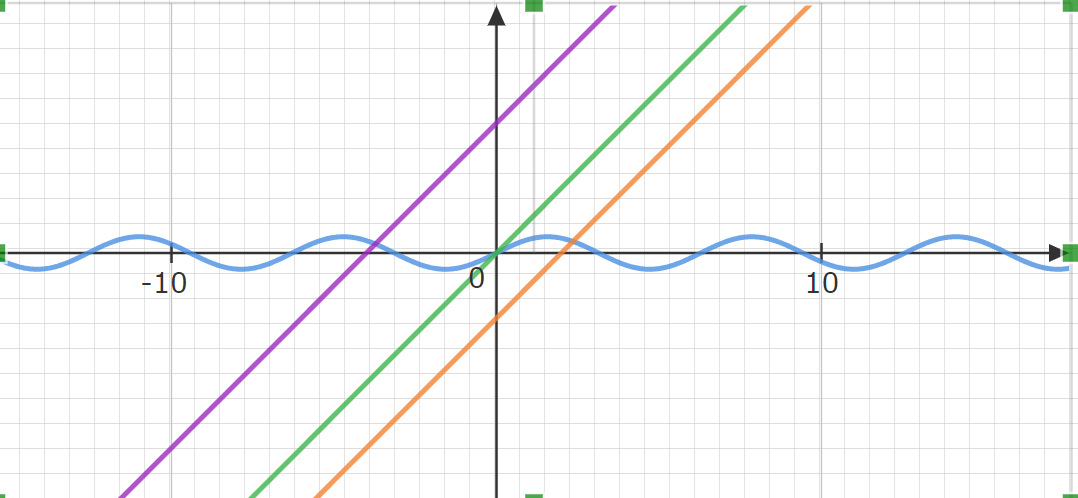
\includegraphics[height=4.9cm,width=8cm]{凸显.PNG}
\centering
\end{figure}

后面的\textit{隐函数存在定理}将严格表明其成立性. 下面是由开普勒方程决定的$y=f(x)$当$\epsilon=0.9$时的图像.


\begin{figure}[h]
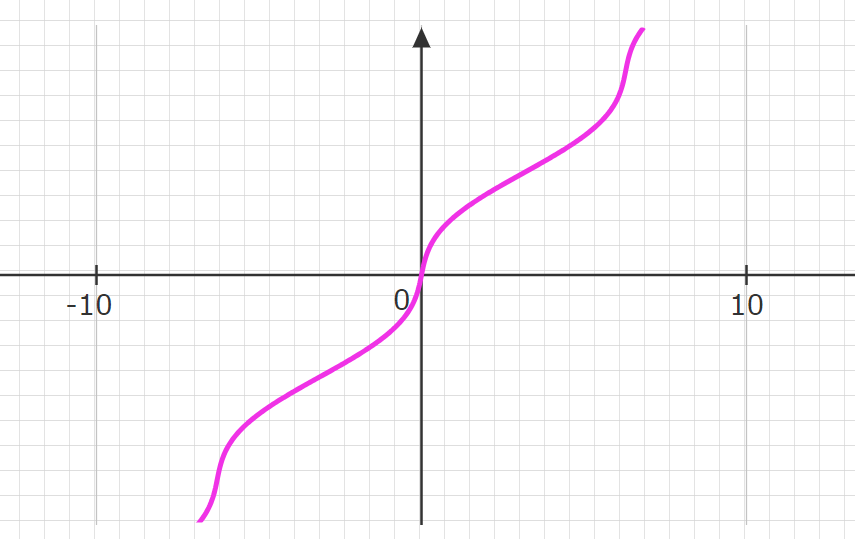
\includegraphics[height=4.9cm,width=8cm]{kepler.PNG}
\centering
\end{figure}

\textbf{例 5.2} 单位圆方程$x^{2}+y^{2}=1$不能直接决定一个函数关系$y=f(x)$,因为一般而言,对某非零$x_{0}$,可能有两个$y$值与之对应. 但我们可取平方根的某一个分支,比如正的,得到$y=\sqrt{1-x^{2}}$,它定义了一个函数关系,其图形是上半圆. 


\newpage

\textbf{例 5.3}方程$x^{3}+x^{2}-y^{2}=0$定义的曲线常被称为\textit{节点曲线(node curve)},其图像见下. 同上例,$y$的正或负平方根定义了一个函数关系. 

\begin{figure}[h]
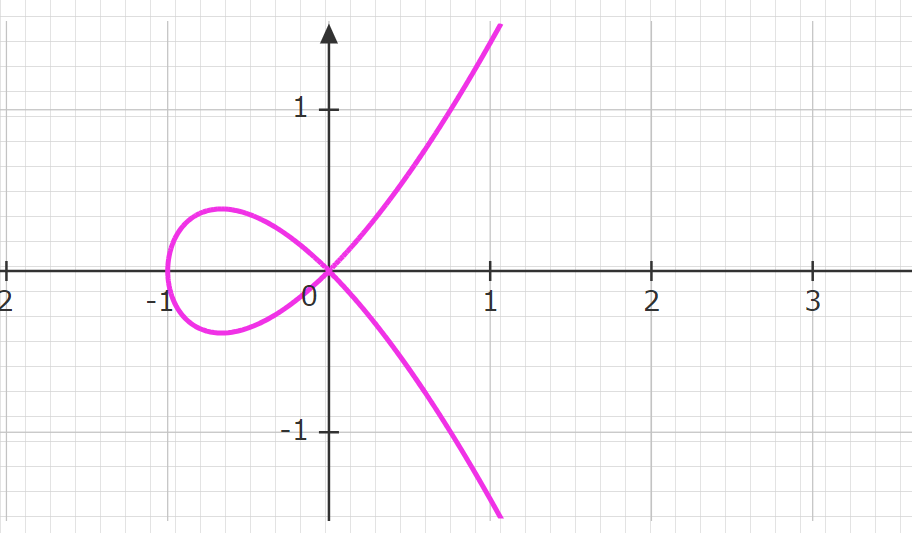
\includegraphics[height=4cm,width=8cm]{node.PNG}
\centering
\caption{\textit{结点曲线}}
\end{figure}

\textbf{例 5.4} 方程$x^{3}-y^{2}=0$定义的曲线常被称为\textit{尖点曲线(cusp curve)},其图像见下. 同上例,$y$的正或负平方根定义了一个函数关系. 


\begin{figure}[h]
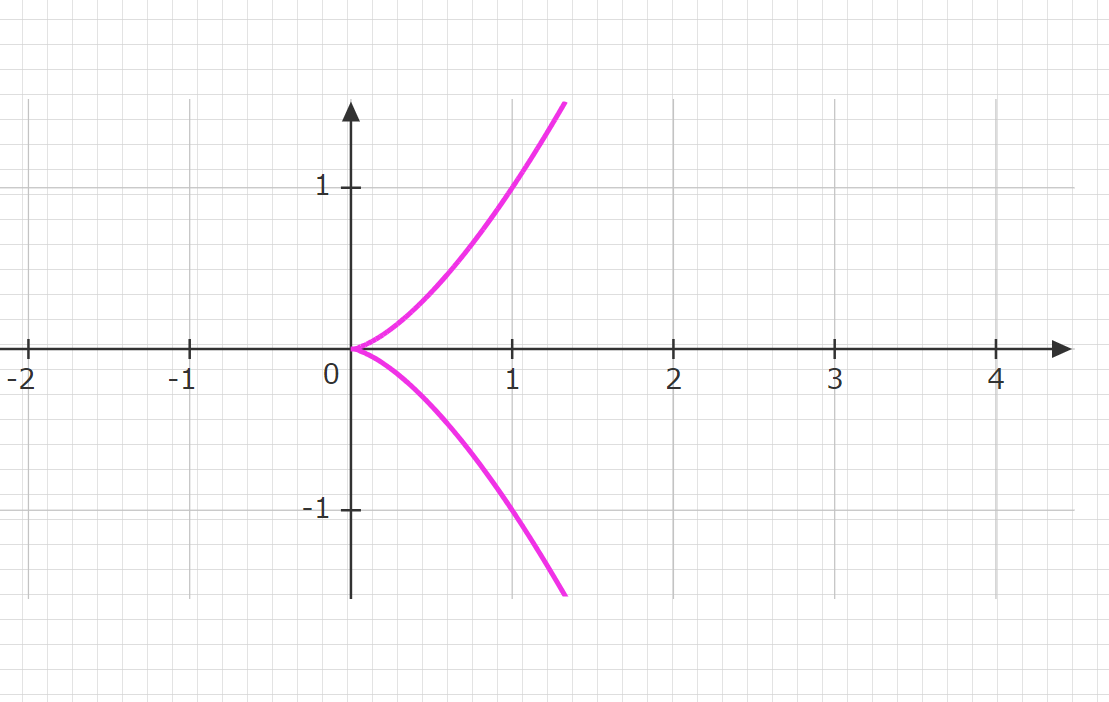
\includegraphics[height=4.2cm,width=8cm]{cusp.PNG}
\centering
\caption{\textit{尖点曲线}}
\end{figure}


\textbf{例 5.5} 方程$y^{2}-x^{3}+x=0$定义的曲线的图形如下,同前,$y$的正或负平方根定义了一个函数关系. 

\begin{figure}[h]
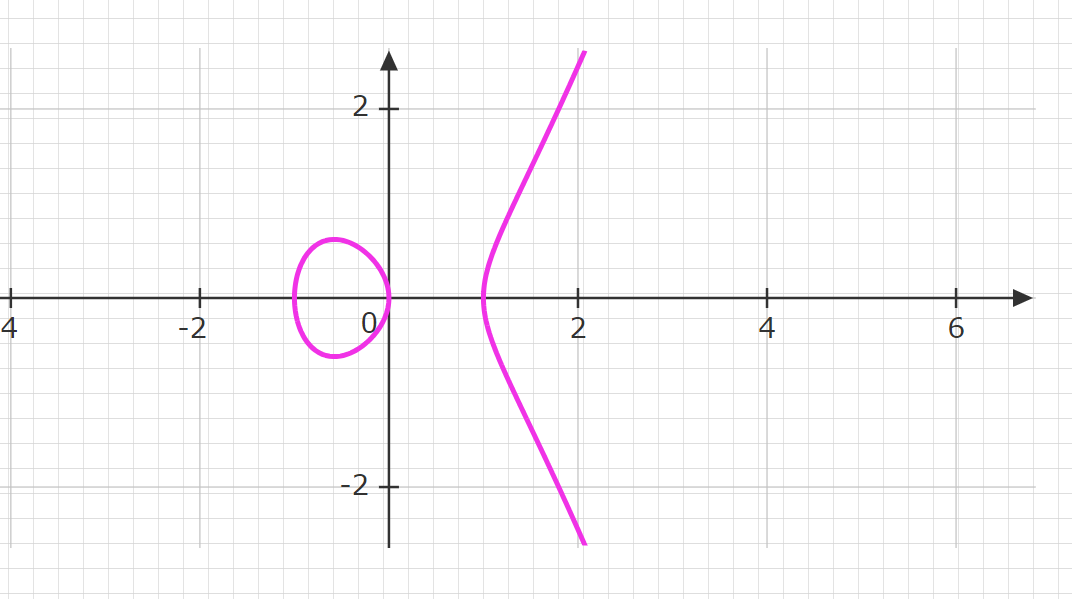
\includegraphics[height=4.2cm,width=8cm]{ellptic.PNG}
\centering
\end{figure}


例$5.3-5.5$都是\textit{椭圆曲线(elliptic curve)}的例子. 

\vspace{3pt}

\textbf{注记 5.1} \textit{更一般地,我们考虑如下形式的方程}\[p_{0}(x)y^{n}+p_{1}(x)y^{n-1}+\cdots+p_{n-1}(x)y+p_{n}(x)=0\]

\textit{其中$p_{i}(x)$都是关于$x$的多项式. 上面的方程决定了平面上的一条\textit{代数曲线(algebraic curve)},由它(通过确定其单值分支)决定的函数称作是\textit{代数函数(algebraic function)}. 显然,多项式函数和有理函数都是代数函数. 不是代数函数的函数称为\textit{超越函数(transcendental function)}. 注意,与实数相比较,多项式相当于整数,有理函数相当于有理数.} 


\vspace{4pt}

设函数由方程$F(x,y)=0$ 给出,若存在一个\textit{参数(parameter)} $t$,使得函数关系可描述为如下方程\[\left\{\begin{array}{c}
     x=x(t)  \\
     y=t(t)
\end{array}\right.\qquad t\in I\subseteq \mathbb{R}\]

则称它是函数的\textit{参数方程(parametric equation)} 表示. 其中参数$t$的取值范围(区间)$I$由原函数的定义域决定. 

\vspace{3pt}

\textbf{注记 5.2} \textit{参数方程表示是比函数更一般的概念:即便$F(x,y)=0$不能界定出函数关系,但我们仍然可以对$F(x,y)=0$描述的曲线进行参数化. }

\vspace{3pt}

\textbf{例 5.6} 对$x^{2}+y^{2}=1$,利用三角函数,有其标准参数方程$\left\{\begin{array}{c}
     x=\cos{t}\\
     y=\sin{t} 
\end{array}\right.\quad t\in \mathbb{R}$. 此时,参数$t$的含义是曲线上点$(x,y)$相对于正$x$-轴的倾角. 当然,也可将$t$解释为“时间”,当$t$从$0$增大到$2\pi$,则曲线上点绕圆逆时针一圈. 当然,参数表达往往有多种表达,比如$x=\cos{2t},\,y=\sin{2t}$ 也是单位圆的参数表达. 与上参数方程的区别是,当时间$t$“流动时”,圆周上点的运动速度不同. 

\vspace{3pt}

如希望参数表达\textbf{例 5.2}中的函数$y=\sqrt{1-x^{2}}\,\,-1\leq x\leq 1$,则只需限制参数$t$的范围. 比如$t\in [-\pi/2,\,\pi/2]$. 

\vspace{3pt}

\textbf{例 5.7} 类似与上例,对椭圆方程$\displaystyle\frac{x^{2}}{a^{2}}+\frac{y^{2}}{b^{2}}=1$,用三角函数给出标准参数方程\[\left\{\begin{array}{c}
     x=a\cos{t}  \\
     y=b\sin{t}
\end{array}\right.\qquad t\in \mathbb{R}\]

\vspace{3pt}

\textbf{例 5.8} 对双曲线$\displaystyle\frac{x^{2}}{a^{2}}-\frac{y^{2}}{b^{2}}=1$,可取其参数方程为$\left\{\begin{array}{c}
     x=\cosh{t} \\
     y=\sinh{t}
\end{array}\right.\quad t\in\mathbb{R}$. 对它的另一种参数方程表示是$\left\{\begin{array}{c}
     x=a sec\,t  \\
     y=b\tan\,t
\end{array}\right.\quad t\in\mathbb{R}$.

\vspace{4pt}

\textbf{例 5.9} \textit{摆线(cycloid)} 是当圆沿直线滚动时,其上一定点$P$的运动轨迹. 设圆半径为$r$,沿$x$轴方向滚动,且$P$的起始位置为原点. 
\begin{center}
    

\tikzset{every picture/.style={line width=0.75pt}} %set default line width to 0.75pt        

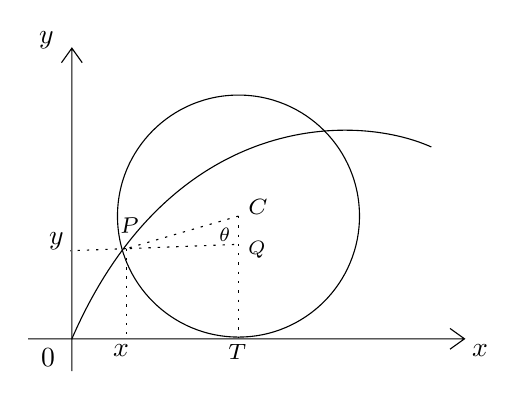
\begin{tikzpicture}[x=0.75pt,y=0.75pt,yscale=-1,xscale=1]
%uncomment if require: \path (0,385); %set diagram left start at 0, and has height of 385

%Shape: Axis 2D [id:dp5564652854867964] 
\draw  (190,230.04) -- (400.2,230.04)(211.02,90) -- (211.02,245.6) (393.2,225.04) -- (400.2,230.04) -- (393.2,235.04) (206.02,97) -- (211.02,90) -- (216.02,97)  ;
%Shape: Circle [id:dp21158302575738985] 
\draw   (233,170.9) .. controls (233,138.7) and (259.1,112.6) .. (291.3,112.6) .. controls (323.5,112.6) and (349.6,138.7) .. (349.6,170.9) .. controls (349.6,203.1) and (323.5,229.2) .. (291.3,229.2) .. controls (259.1,229.2) and (233,203.1) .. (233,170.9) -- cycle ;
%Straight Lines [id:da2654857563296258] 
\draw  [dash pattern={on 0.84pt off 2.51pt}]  (291.3,170.9) -- (291.3,229.2) ;
%Curve Lines [id:da8107822423549713] 
\draw    (211.02,230.04) .. controls (258.2,121.6) and (346.2,120.6) .. (384.2,137.6) ;
%Straight Lines [id:da15479601871740423] 
\draw  [dash pattern={on 0.84pt off 2.51pt}]  (291.3,170.9) -- (237.2,186.6) ;
%Straight Lines [id:da5739200290724504] 
\draw  [dash pattern={on 0.84pt off 2.51pt}]  (289.2,184.6) -- (237.2,186.6) ;
%Straight Lines [id:da5051780423687366] 
\draw  [dash pattern={on 0.84pt off 2.51pt}]  (237.2,186.6) -- (237.2,229.6) ;
%Straight Lines [id:da40966226799770245] 
\draw  [dash pattern={on 0.84pt off 2.51pt}]  (237.2,186.6) -- (210.2,187.6) ;

% Text Node
\draw (403,231.4) node [anchor=north west][inner sep=0.75pt]    {$x$};
% Text Node
\draw (194,80.4) node [anchor=north west][inner sep=0.75pt]    {$y$};
% Text Node
\draw (195,233.4) node [anchor=north west][inner sep=0.75pt]    {$0$};
% Text Node
\draw (285,231.4) node [anchor=north west][inner sep=0.75pt]  [font=\footnotesize]  {$T$};
% Text Node
\draw (232.71,170.73) node [anchor=north west][inner sep=0.75pt]  [font=\footnotesize,rotate=-356.93]  {$P$};
% Text Node
\draw (295,161.4) node [anchor=north west][inner sep=0.75pt]  [font=\footnotesize]  {$C$};
% Text Node
\draw (295,181.4) node [anchor=north west][inner sep=0.75pt]  [font=\scriptsize]  {$Q$};
% Text Node
\draw (281,175.4) node [anchor=north west][inner sep=0.75pt]  [font=\scriptsize]  {$\theta $};
% Text Node
\draw (230,231.4) node [anchor=north west][inner sep=0.75pt]    {$x$};
% Text Node
\draw (199,177.4) node [anchor=north west][inner sep=0.75pt]    {$y$};


\end{tikzpicture}
\end{center}

记$\theta$为圆滚动时转过的角度,由上图知$\overline{OT}=\overset{\frown}{PT}=r\theta$. 而动点$P$的坐标$(x,y)$满足下约束\[\left\{\begin{array}{c}
     x=\overline{OT}-\overline{PQ}  \\
     y=\overline{TC}-\overline{QC}
\end{array}\right.\quad \Longrightarrow\quad \left\{\begin{array}{c}
     x=r\theta-r\sin{\theta}  \\
     y=r-r\sin{\theta}
\end{array}\right.\quad \theta\in\mathbb{R}\]

摆线是周期曲线,它的一个基本周期对应参数$0\leq \theta\leq 2\pi$

\begin{center}
    

\tikzset{every picture/.style={line width=0.75pt}} %set default line width to 0.75pt        

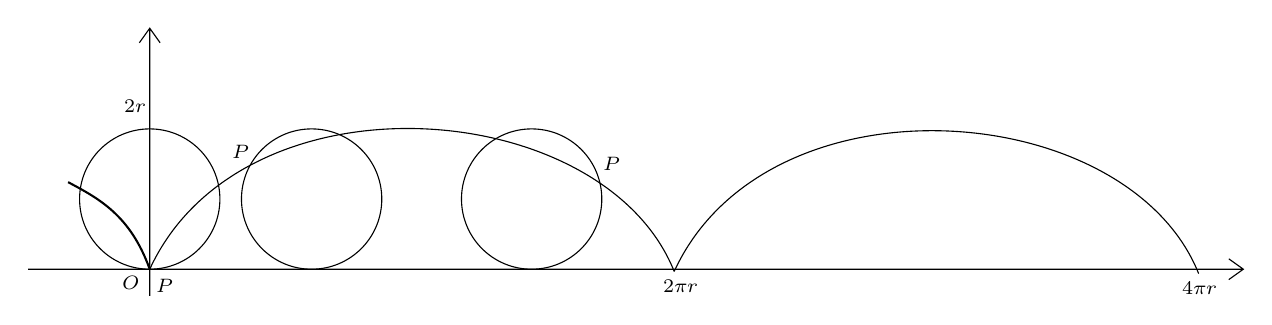
\begin{tikzpicture}[x=0.75pt,y=0.75pt,yscale=-1,xscale=1]
%uncomment if require: \path (0,385); %set diagram left start at 0, and has height of 385

%Shape: Axis 2D [id:dp9164828448857585] 
\draw  (124.98,290.54) -- (710.41,290.54)(183.52,174.44) -- (183.52,303.44) (703.41,285.54) -- (710.41,290.54) -- (703.41,295.54) (178.52,181.44) -- (183.52,174.44) -- (188.52,181.44)  ;
%Shape: Circle [id:dp8273945219697361] 
\draw   (149.72,256.74) .. controls (149.72,238.07) and (164.85,222.94) .. (183.52,222.94) .. controls (202.19,222.94) and (217.32,238.07) .. (217.32,256.74) .. controls (217.32,275.41) and (202.19,290.54) .. (183.52,290.54) .. controls (164.85,290.54) and (149.72,275.41) .. (149.72,256.74) -- cycle ;
%Shape: Circle [id:dp4655777862201924] 
\draw   (227.72,256.74) .. controls (227.72,238.07) and (242.85,222.94) .. (261.52,222.94) .. controls (280.19,222.94) and (295.32,238.07) .. (295.32,256.74) .. controls (295.32,275.41) and (280.19,290.54) .. (261.52,290.54) .. controls (242.85,290.54) and (227.72,275.41) .. (227.72,256.74) -- cycle ;
%Shape: Circle [id:dp3057788087272779] 
\draw   (333.72,256.74) .. controls (333.72,238.07) and (348.85,222.94) .. (367.52,222.94) .. controls (386.19,222.94) and (401.32,238.07) .. (401.32,256.74) .. controls (401.32,275.41) and (386.19,290.54) .. (367.52,290.54) .. controls (348.85,290.54) and (333.72,275.41) .. (333.72,256.74) -- cycle ;
%Curve Lines [id:da08536547848800646] 
\draw [line width=0.75]    (144.2,248.6) .. controls (159.2,256.6) and (174.2,264.6) .. (183.52,290.54) ;
%Curve Lines [id:da3739955518512028] 
\draw    (183.52,290.54) .. controls (228.2,193.6) and (402.2,206.6) .. (436.2,291.6) ;
%Curve Lines [id:da11963755942968413] 
\draw    (436.2,291.6) .. controls (480.88,194.66) and (654.88,207.66) .. (688.88,292.66) ;

% Text Node
\draw (169,292.4) node [anchor=north west][inner sep=0.75pt]  [font=\scriptsize]  {$O$};
% Text Node
\draw (185.52,293.94) node [anchor=north west][inner sep=0.75pt]  [font=\scriptsize]  {$P$};
% Text Node
\draw (222,229.4) node [anchor=north west][inner sep=0.75pt]  [font=\scriptsize]  {$P$};
% Text Node
\draw (401,235.4) node [anchor=north west][inner sep=0.75pt]  [font=\scriptsize]  {$P$};
% Text Node
\draw (170,207.4) node [anchor=north west][inner sep=0.75pt]  [font=\scriptsize]  {$2r$};
% Text Node
\draw (430,294.4) node [anchor=north west][inner sep=0.75pt]  [font=\scriptsize]  {$2\pi r$};
% Text Node
\draw (680,295.4) node [anchor=north west][inner sep=0.75pt]  [font=\scriptsize]  {$4\pi r$};


\end{tikzpicture}
\end{center}

\textbf{例 5.6$^{\prime}$} 由于三角函数是超越函数,故例 5.6 中对单位圆的标准参数化是超越参数化,自然,它相当于用过原点的旋转直线族与圆周相交,然后利用$\theta$来标记点的位置. 在现实应用中(尤其在数论问题中)我们希望能够代数地参数曲线,即用参数的有理函数来表达变量. 
\begin{center}
    

\tikzset{every picture/.style={line width=0.75pt}} %set default line width to 0.75pt        

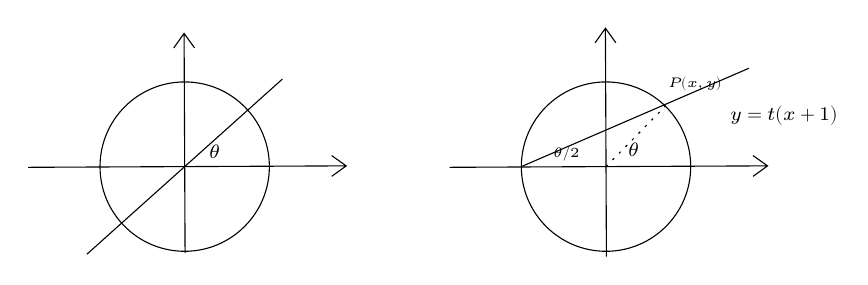
\begin{tikzpicture}[x=0.75pt,y=0.75pt,yscale=-1,xscale=1]
%uncomment if require: \path (0,385); %set diagram left start at 0, and has height of 385

%Shape: Axis 2D [id:dp08532478292403667] 
\draw  (163.01,239.31) -- (316.21,238.61)(238.1,174.78) -- (238.58,280.7) (309.19,233.65) -- (316.21,238.61) -- (309.24,243.65) (233.13,181.81) -- (238.1,174.78) -- (243.13,181.76)  ;
%Shape: Circle [id:dp15445500527664202] 
\draw   (197.59,238.97) .. controls (197.59,216.43) and (215.85,198.17) .. (238.39,198.17) .. controls (260.92,198.17) and (279.19,216.43) .. (279.19,238.97) .. controls (279.19,261.5) and (260.92,279.77) .. (238.39,279.77) .. controls (215.85,279.77) and (197.59,261.5) .. (197.59,238.97) -- cycle ;
%Straight Lines [id:da7537380392467592] 
\draw    (191.29,281.17) -- (285.49,196.77) ;
%Shape: Axis 2D [id:dp6272102782533355] 
\draw  (366.01,239.31) -- (519.21,238.61)(441.09,172.3) -- (441.58,282.31) (512.19,233.65) -- (519.21,238.61) -- (512.24,243.65) (436.12,179.33) -- (441.09,172.3) -- (446.12,179.28)  ;
%Shape: Circle [id:dp08789856101461369] 
\draw   (400.59,238.97) .. controls (400.59,216.43) and (418.85,198.17) .. (441.39,198.17) .. controls (463.92,198.17) and (482.19,216.43) .. (482.19,238.97) .. controls (482.19,261.5) and (463.92,279.77) .. (441.39,279.77) .. controls (418.85,279.77) and (400.59,261.5) .. (400.59,238.97) -- cycle ;
%Straight Lines [id:da635134825730733] 
\draw    (400.59,238.97) -- (510.2,191.6) ;
%Straight Lines [id:da767790624544584] 
\draw  [dash pattern={on 0.84pt off 2.51pt}]  (441.39,238.97) -- (470.2,209.6) ;

% Text Node
\draw (249,227.4) node [anchor=north west][inner sep=0.75pt]  [font=\scriptsize]  {$\theta $};
% Text Node
\draw (451,226.4) node [anchor=north west][inner sep=0.75pt]  [font=\scriptsize]  {$\theta $};
% Text Node
\draw (415,228.4) node [anchor=north west][inner sep=0.75pt]  [font=\tiny]  {$\theta /2$};
% Text Node
\draw (500,208.4) node [anchor=north west][inner sep=0.75pt]  [font=\scriptsize]  {$y=t( x+1)$};
% Text Node
\draw (470,194.4) node [anchor=north west][inner sep=0.75pt]  [font=\tiny]  {$P( x,y)$};

\end{tikzpicture}
\end{center}

过点$(-1,0)$的旋转直线族$y=t(x+1),\,t\in\mathbb{R}$ 与圆$x^{2}+y^{2}=1$相交. 交点$P(x,y)$的坐标满足\[\left\{\begin{array}{c}
     x^{2}+y^{2}=1  \\
     y=t(x+1)
\end{array}\right.\quad \Longrightarrow\quad \left\{\begin{array}{c}
     x=\frac{1-t^{2}}{1+t^{2}}  \\
    y=\frac{2t}{1+t^{2}} 
\end{array}\right.\quad t\in \mathbb{R}\]

此即为单位圆的有理参数化. 参数$t$的含义是直线族的斜率. 注意到$t=\tan\frac{\theta}{2}$,故上有理参数化给出了三角函数的“万能公式”\[\cos{\theta}=\frac{1-\tan^{2}\frac{\theta}{2}}{1+\tan^{2}\frac{\theta}{2}}\qquad \quad \sin\theta=\frac{2\tan\frac{\theta}{2}}{1+\tan^{2}\frac{\theta}{2}}\]

\textbf{注记 5.3} \textit{由单位圆的有理参数化,可给出方程$x^{2}+y^{2}=z^{2}$的所有整数解. 即令}\[\frac{x}{z}=\frac{1-t^{2}}{1+t^{2}};\qquad \frac{y}{z}=\frac{2t}{1+t^{2}}\]

\textit{令$t$遍历所有整数,则$  x=1-t^{2};\,y=2t;\,z=1+t^{2}$给出所有整数解.}

\vspace{3pt}

\textbf{例 5.3$^{\prime}$} 由\textit{例 5.3} 中\textit{节点曲线}$x^{3}+x^{2}-y^{2}=0$的图形知,我们可利用过原点的旋转直线族给出其有理参数,即解方程组\[\left\{\begin{array}{c}
x^{3}+x^{2}-y^{2}=0  \\
     y=tx
\end{array}\right.\quad \Longrightarrow\quad \left\{\begin{array}{c}
    x=t^{2}-1  \\
     y=t^{3}-t
\end{array}\right.\quad t\in \mathbb{R}\]

\begin{center}


\tikzset{every picture/.style={line width=0.75pt}} %set default line width to 0.75pt        

\begin{tikzpicture}[x=0.75pt,y=0.75pt,yscale=-1,xscale=1]
%uncomment if require: \path (0,385); %set diagram left start at 0, and has height of 385

%Curve Lines [id:da1159820514860983] 
\draw    (342.2,82.6) .. controls (238.2,312.6) and (194.2,-5.4) .. (361.2,207.6) ;
%Straight Lines [id:da8029910507752092] 
\draw  [dash pattern={on 0.84pt off 2.51pt}]  (221.2,129.6) -- (382.2,166.6) ;
%Straight Lines [id:da39442915872636686] 
\draw  [dash pattern={on 0.84pt off 2.51pt}]  (218.2,152.6) -- (389.2,144.6) ;
%Straight Lines [id:da32345605933119925] 
\draw  [dash pattern={on 0.84pt off 2.51pt}]  (214.2,175.1) -- (388.2,122.6) ;


\end{tikzpicture}
\end{center}


\section{极坐标与极坐标下的曲线描述}

平面上点$P$的位置除用笛卡尔坐标$(x,y)$表示外,还可用\textit{极坐标(polar coordinate)}$(r,\theta)$来表示. 极坐标与笛卡尔坐标之间的转换关系为\[\left\{\begin{array}{c}
     x=r\cos{\theta} \\
     y=r\sin{\theta}
\end{array}\right.\qquad \Longleftrightarrow\qquad\left\{\begin{array}{c}
     r=\sqrt{x^{2}+y^{2}}  \\
     \theta=\arctan\frac{y}{x}\quad \textit{第一象限内}
\end{array}\right.\]

\begin{center}
    

\tikzset{every picture/.style={line width=0.75pt}} %set default line width to 0.75pt        

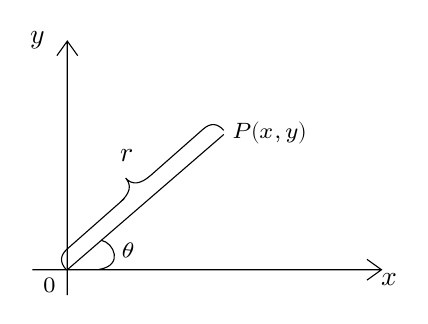
\begin{tikzpicture}[x=0.75pt,y=0.75pt,yscale=-1,xscale=1]
%uncomment if require: \path (0,385); %set diagram left start at 0, and has height of 385

%Shape: Axis 2D [id:dp6423134348156787] 
\draw  (284,232.76) -- (452.2,232.76)(300.82,122.6) -- (300.82,245) (445.2,227.76) -- (452.2,232.76) -- (445.2,237.76) (295.82,129.6) -- (300.82,122.6) -- (305.82,129.6)  ;
%Straight Lines [id:da44957534638985863] 
\draw    (376.2,167.6) -- (300.82,232.76) ;
%Curve Lines [id:da4447636248636522] 
\draw    (317.2,218.6) .. controls (323.2,219.6) and (328.2,230.6) .. (316.2,232.6) ;
%Shape: Brace [id:dp42590438753482984] 
\draw   (376.2,165.6) .. controls (373.11,162.1) and (369.82,161.89) .. (366.32,164.98) -- (341.07,187.24) .. controls (336.07,191.65) and (332.03,192.1) .. (328.94,188.6) .. controls (332.03,192.1) and (331.07,196.05) .. (326.07,200.46)(328.32,198.48) -- (300.82,222.72) .. controls (297.32,225.81) and (297.11,229.1) .. (300.2,232.6) ;

% Text Node
\draw (451,233.4) node [anchor=north west][inner sep=0.75pt]    {$x$};
% Text Node
\draw (282,116.4) node [anchor=north west][inner sep=0.75pt]    {$y$};
% Text Node
\draw (288,235.4) node [anchor=north west][inner sep=0.75pt]  [font=\footnotesize]  {$0$};
% Text Node
\draw (379,160.4) node [anchor=north west][inner sep=0.75pt]  [font=\footnotesize]  {$P( x,y)$};
% Text Node
\draw (326.53,217.88) node [anchor=north west][inner sep=0.75pt]  [font=\footnotesize,rotate=-5.17]  {$\theta $};
% Text Node
\draw (325,173.4) node [anchor=north west][inner sep=0.75pt]    {$r$};


\end{tikzpicture}
\end{center}

在极坐标下,平面曲线$F(x,y)=0$ 可表示为$G(r,\theta)=0$,即由$r$ 和$\theta$的关系$G$给出. 若曲线显式表达为$r=r(\theta)$,根据$\theta$的取值范围,可描绘出曲线的形状. 

\vspace{3pt}


\textbf{例 6.1} $r=c$(其中$c>0$ 为常数) 描述了圆心为原点,半径为$c$的圆;$\theta=c$(其中$\theta\neq 0$为常数),给出过原点的,以 $\theta$为倾斜角的射线. 

\vspace{3pt}

\textbf{注 6.1} \textit{若曲线由$r=r(\theta),\,\theta\in I$给出,则有自然参数化}$\left\{\begin{array}{c}
     x=r(\theta)\cos\theta  \\
     y=r(\theta)\sin\theta
\end{array}\right.\quad\theta\in I$. \textit{如$x^{2}+y^{2}=4$的极坐标方程是$r=2$,可得参数方程$\left\{\begin{array}{c}
     x=2\cos{\theta}  \\
     y=2\sin{\theta}
\end{array}\right.$}

\vspace{6pt}

\textbf{例 6.2} 直线$x+y=1$的极坐标方程为$r=\frac{2}{\sin{\theta}+\cos{\theta}}$,为使$r\geq 0$,可取$\theta\in\left(-\frac{\pi}{4},\,\frac{3\pi}{4}\right) $.

\vspace{3pt}

\textbf{例 6.3} 设曲线由方程$(x^{2}+y^{2})^{2}=a^{2}(x^{2}-y^{2})\,(a>0)$给出,则在极坐标下,有$r=a\sqrt{\cos{2\theta}}$. 只需考察在一个周期$\theta\in \left[-\frac{\pi}{2},\,\frac{3\pi}{2}\right]$ 内的情形. 由于$\cos{2\theta}\geq 0$,故$\theta$的取值被限制为$\theta\in \left[-\frac{\pi}{4},\,\frac{\pi}{4}\right]\cup \left[\frac{3\pi}{4},\,\frac{5\pi}{4}\right]$. 由此可绘制出曲线的图形如下
\begin{center}
    

\begin{figure}[h]
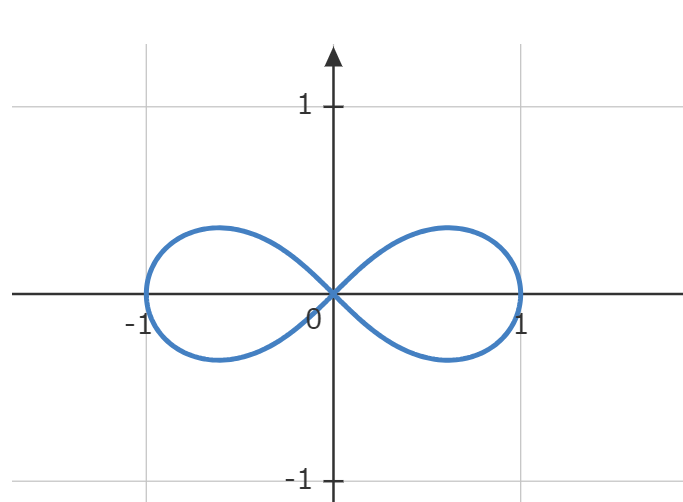
\includegraphics[height=3cm,width=4.5cm]{8.PNG}
\centering
\caption{\textit{双扭线}}
\end{figure}
\end{center}

\textbf{例 6.4} 极坐标下的方程$r=a\cos{n\theta}$($a>0,\,n\in \mathbb{N}^{+}$)描述的封闭曲线是多叶型的,当$n$是奇数时,叶子的个数是$n$;当$n$是偶数时,叶子的个数是$2n$. 下面是一些例子.

\begin{figure}[htbp]
  \subfigure[$n=2$]{
    \begin{minipage}[t]{0.4\textwidth}
      \centering
      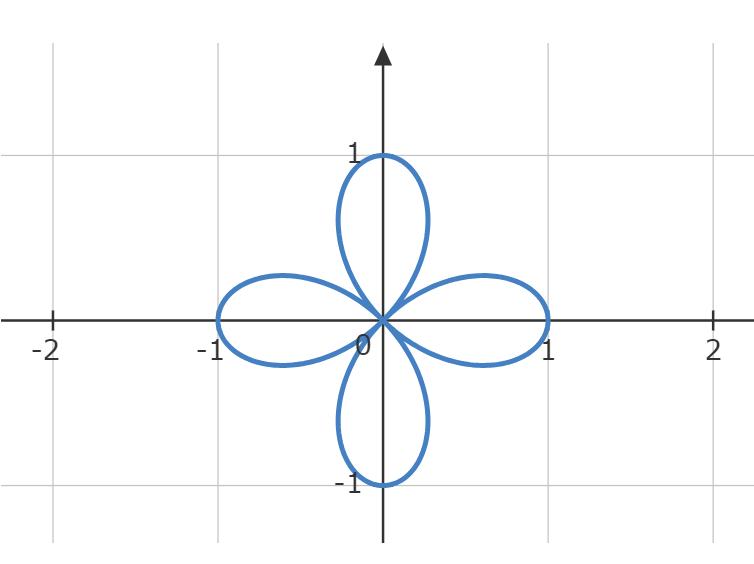
\includegraphics[width=\textwidth]{4pedal.PNG}
    \end{minipage}
  }
  \hfill
  \subfigure[$n=3$]{
    \begin{minipage}[t]{0.4\textwidth}
      \centering
      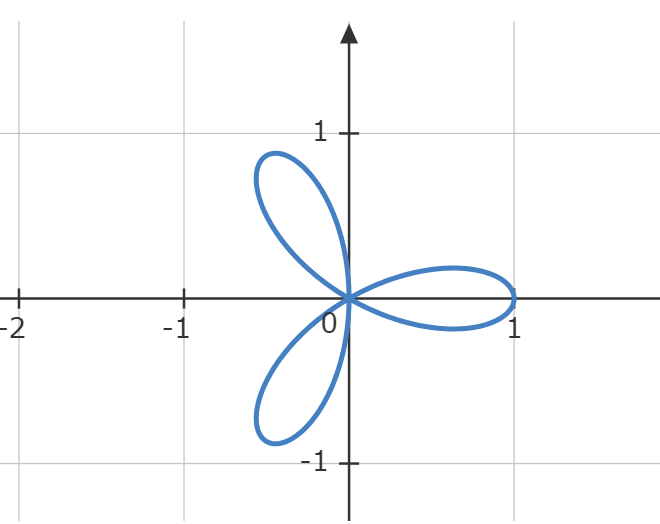
\includegraphics[width=\textwidth]{3pedal.PNG}
    \end{minipage}
  }
\end{figure}

\begin{figure}[htbp]
  \subfigure[$n=4$]{
    \begin{minipage}[t]{0.4\textwidth}
      \centering
      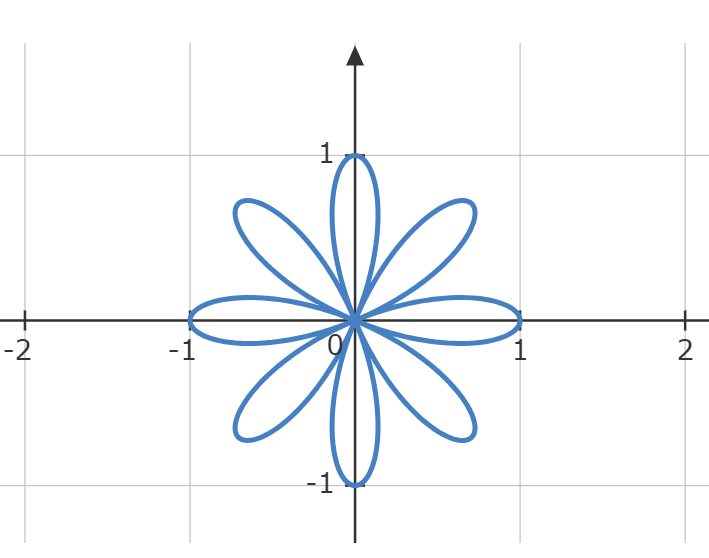
\includegraphics[width=\textwidth]{8pedal.PNG}
    \end{minipage}
  }
  \hfill
  \subfigure[$n=5$]{
    \begin{minipage}[t]{0.4\textwidth}
      \centering
      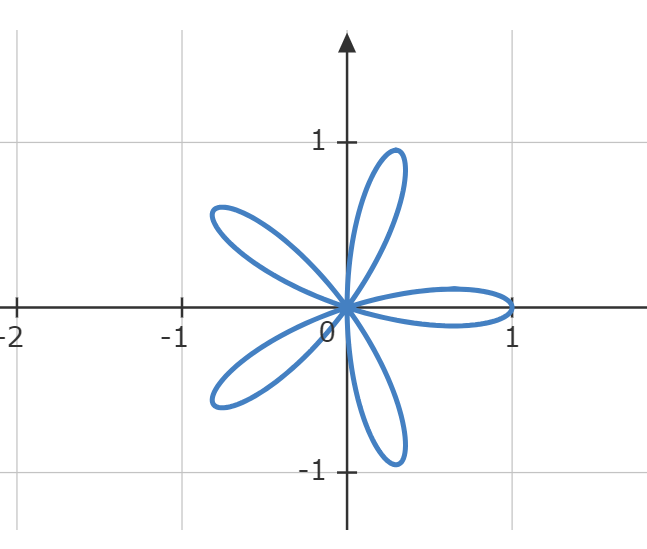
\includegraphics[width=\textwidth]{5 pedal.PNG}
    \end{minipage}
  }

\end{figure}



\newpage





\section{附:不用极限的求导之多项式函数的导数}

微分学主要研究函数在一点临近的性质. 更具体说,我们希望在一点附近,用一个线性映射来\textit{逼近(approximate)}函数. 

\vspace{4pt}

给定一函数$y=f(x)$,它定义了从其定义域$D(f)$到其值域$R(f)$的一个映射. 在$x_{0}\in D(f)$ 附近,若函数有足够的\textit{光滑性(smoothness)——切线存在},可用其在$x_{0}$点出的切线来近似$f(x)$. 设切线方程是$y-f(x_{0})=k(x-x_{0})$(\textit{后面会知道,斜率$k=f^{\prime}(x_{0})$} 是$f(x)$在$x_{0}$处的导数),记它定义的映射为\[T_{f}(x_{0}): x\longmapsto f(x_{0})+f^{\prime}(x_{0})(x-x_{0})\]

当$x$足够接近$x_{0}$时,$T_{f}(x_{0})$通常是$f(x)$在$x_{0}$附近的一个好的近似. \[f(x)\approx T_{f}(x_{0})\quad x\,\textit{接近}\,x_{0}\]

由$T_{f}(x_{0})$界定的\textit{线性映射}$L_{f}(x_{0}):\,u\longmapsto f^{\prime}(x_{0})u\,(u:=x-x_{0})$ 称为函数$f(x)$在$x_{0}$处的\textit{微分(differential)}. 它是函数在$x=x_{0}$附近变化的\textit{线性主部}.

\begin{center}
    

\tikzset{every picture/.style={line width=0.75pt}} %set default line width to 0.75pt        

\begin{tikzpicture}[x=0.75pt,y=0.75pt,yscale=-1,xscale=1]
%uncomment if require: \path (0,385); %set diagram left start at 0, and has height of 385

%Shape: Axis 2D [id:dp7999999264744655] 
\draw  (67,233.6) -- (331.2,233.6)(98.2,56.6) -- (98.2,257) (324.2,228.6) -- (331.2,233.6) -- (324.2,238.6) (93.2,63.6) -- (98.2,56.6) -- (103.2,63.6)  ;
%Curve Lines [id:da861835112564107] 
\draw    (86.2,211.6) .. controls (97.2,188.6) and (126.2,56.6) .. (314.2,190.6) ;
%Straight Lines [id:da8661919348463805] 
\draw    (55,167) -- (310.2,80.6) ;
%Straight Lines [id:da8266093647008306] 
\draw  [dash pattern={on 0.84pt off 2.51pt}]  (149.2,136.6) -- (150.2,232.6) ;

% Text Node
\draw (328,237.4) node [anchor=north west][inner sep=0.75pt]    {$x$};
% Text Node
\draw (82,47.4) node [anchor=north west][inner sep=0.75pt]    {$y$};
% Text Node
\draw (83,237.4) node [anchor=north west][inner sep=0.75pt]    {$0$};
% Text Node
\draw (334,184.4) node [anchor=north west][inner sep=0.75pt]    {$y=f( x)$};
% Text Node
\draw (143,237.4) node [anchor=north west][inner sep=0.75pt]    {$x_{0}$};
% Text Node
\draw (294,93.4) node [anchor=north west][inner sep=0.75pt]    {$y-f( x_{0}) =\underbrace{f^{\prime }( x_{0})( x-x_{0})}_{L_{f}(x_{0})}$};

\end{tikzpicture}
\end{center}

而我们知道,曲线在一点处的切线,直观上来讲,是过这点,且在这点\textbf{附近}与曲线仅交与该点的直线. 由此,我们可以对简单的多项式函数“求导”,而无需知道导数的定义. 

\vspace{3pt}

比如对二次曲线$y=x^{2}+3x+1$,为求其在$(0,1)$处的切线,我们考虑过该点的直线族$y=kx+1$,并求解\[\left\{\begin{array}{c}
     y=x^{2}+3x+1  \\
     y=kx+1
\end{array}\right.\quad \Longrightarrow\quad x^{2}+(3-k)x=0\]

当且仅当$k=3$时,有唯一交点$(0,1)$,故$(0,1)$处的切线方程为$y=3x+1$,它刚好是$x^{2}+3x+1$的线性部分,凸显微分是函数变化线性主部的意义. 即在点$(0,1)$附近,映射$y=f(x)$在局部可由线性映射(函数在$x=0$处的微分)$x\longmapsto 3x+1$ 近似. 

\vspace{3pt}

用同样的方法,可求出曲线在$x=1$处的切线方程为$y=5x$. 但我们可以更简单地求解如下:

\vspace{3pt}

在点$x=1$附件,更好的“坐标”是$u=x-1$(恰如$x$是$x=0$处的“好”坐标). 可将$y=x^{2}+3x+1$用$u=x-1$改写为
\[y=(x-1+1)^{2}+3(x-1+1)+1=(x-1)^{2}+5(x-1)+5\]

其线性部分$5(x-1)+5=5x$即为所求切线方程. 同理,为聚焦函数在$x=-1$处的表现,我们用局部坐标$u=x+1$改写函数\[y=x^{2}+3x+1=(x+1-1)^{2}+3(x+1-1)+1=(x+1)^{2}+(x+1)-1\]

其线性部分$x+1-1=x$必为$x=-1$处的切线方程. 

\begin{figure}[h]
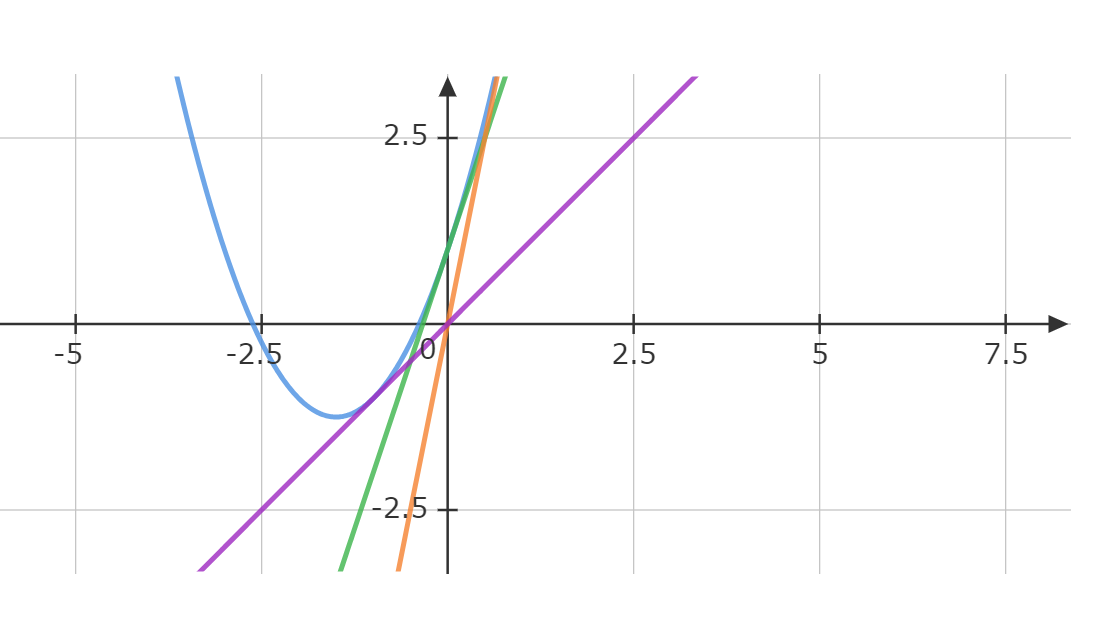
\includegraphics[height=6cm,width=10cm]{de.PNG}
\centering
\end{figure}







\end{document}
